\documentclass[12pt,english]{article}\usepackage[]{graphicx}\usepackage[]{color}
%% maxwidth is the original width if it is less than linewidth
%% otherwise use linewidth (to make sure the graphics do not exceed the margin)
\makeatletter
\def\maxwidth{ %
  \ifdim\Gin@nat@width>\linewidth
    \linewidth
  \else
    \Gin@nat@width
  \fi
}
\makeatother

\definecolor{fgcolor}{rgb}{0.345, 0.345, 0.345}
\newcommand{\hlnum}[1]{\textcolor[rgb]{0.686,0.059,0.569}{#1}}%
\newcommand{\hlstr}[1]{\textcolor[rgb]{0.192,0.494,0.8}{#1}}%
\newcommand{\hlcom}[1]{\textcolor[rgb]{0.678,0.584,0.686}{\textit{#1}}}%
\newcommand{\hlopt}[1]{\textcolor[rgb]{0,0,0}{#1}}%
\newcommand{\hlstd}[1]{\textcolor[rgb]{0.345,0.345,0.345}{#1}}%
\newcommand{\hlkwa}[1]{\textcolor[rgb]{0.161,0.373,0.58}{\textbf{#1}}}%
\newcommand{\hlkwb}[1]{\textcolor[rgb]{0.69,0.353,0.396}{#1}}%
\newcommand{\hlkwc}[1]{\textcolor[rgb]{0.333,0.667,0.333}{#1}}%
\newcommand{\hlkwd}[1]{\textcolor[rgb]{0.737,0.353,0.396}{\textbf{#1}}}%
\let\hlipl\hlkwb

\usepackage{framed}
\makeatletter
\newenvironment{kframe}{%
 \def\at@end@of@kframe{}%
 \ifinner\ifhmode%
  \def\at@end@of@kframe{\end{minipage}}%
  \begin{minipage}{\columnwidth}%
 \fi\fi%
 \def\FrameCommand##1{\hskip\@totalleftmargin \hskip-\fboxsep
 \colorbox{shadecolor}{##1}\hskip-\fboxsep
     % There is no \\@totalrightmargin, so:
     \hskip-\linewidth \hskip-\@totalleftmargin \hskip\columnwidth}%
 \MakeFramed {\advance\hsize-\width
   \@totalleftmargin\z@ \linewidth\hsize
   \@setminipage}}%
 {\par\unskip\endMakeFramed%
 \at@end@of@kframe}
\makeatother

\definecolor{shadecolor}{rgb}{.97, .97, .97}
\definecolor{messagecolor}{rgb}{0, 0, 0}
\definecolor{warningcolor}{rgb}{1, 0, 1}
\definecolor{errorcolor}{rgb}{1, 0, 0}
\newenvironment{knitrout}{}{} % an empty environment to be redefined in TeX

\usepackage{alltt}
\usepackage{natbib}
\usepackage{amsmath,mathtools,amssymb,mathrsfs,dsfont,amsthm}
\usepackage[margin=1in]{geometry}
%% \usepackage{algpseudocode}
%% \usepackage{algorithm}
\usepackage{caption}
\renewcommand\thefigure{\Alph{figure}}

\usepackage[T1]{fontenc}
\usepackage{babel}
\usepackage{graphicx}
\usepackage{float}
\usepackage{color}
\usepackage{subcaption}
\graphicspath{ {figs/} }
\usepackage[colorlinks]{hyperref}
\hypersetup{citecolor=blue}
\usepackage{enumitem}
\usepackage{authblk}
\usepackage{lineno}
\usepackage[normalem]{ulem}

\usepackage{float}

\usepackage[toc,page]{appendix}

% !Rnw weave = knitr

\renewcommand\Affilfont{\itshape\scriptsize}
\renewcommand\Authfont{\small}

\DeclareCaptionFormat{algor}{%
  \hrulefill\par\offinterlineskip\vskip1pt%
  \textbf{#1#2}#3\offinterlineskip\hrulefill}
\DeclareCaptionStyle{algori}{singlelinecheck=off,format=algor,labelsep=space}
\captionsetup[algorithm]{style=algori}

\def\thesection{S\arabic{section}}
\IfFileExists{upquote.sty}{\usepackage{upquote}}{}
\begin{document}


\author[1,2,3]{Oliver M. Crook}
\author[2]{Claire M. Mulvey}
\author[3]{Paul D.W. Kirk}
\author[2]{Kathryn S. Lilley}
\author[1,2,4,*]{Laurent Gatto}



\affil[1]{Computational Proteomics Unit, Department of
  Biochemistry, University of Cambridge, Cambridge, UK}
\affil[2]{Cambridge Centre for Proteomics, Department of Biochemistry,
  University of Cambridge, Cambridge, UK}
\affil[3]{MRC Biostatistics Unit, Cambridge Institute for Public
  Health, Cambridge, UK}
\affil[4]{Current address: de Duve Institute, UCLouvain, Avenue
  Hippocrate 75, 1200 Brussels, Belgium}
\affil[*]{\url{laurent.gatto@uclouvain.be}}


\title{Supporting information for A Bayesian Mixture Modelling Approach For Spatial Proteomics}

\date{}

\maketitle





\section{Derivation of EM algorithm for TAGM model}\label{apd:EMderv}

This appendix give a formal derivation of the EM algorithm used for
our model. Computations are standard but useful and similar technical
summaries can be found (for example see \cite{Fraley:2005,
  Murphy:2007}) We let
$H = \{\boldsymbol{\mu}_0, \lambda_0, \nu_0, S_0\}$ denote the
parameters of the normal-inverse-Wishart prior. More precisely:

\begin{equation} \label{equation::prior}
\boldsymbol{\mu}_k, \Sigma_k\sim \mathcal{N}\left(\boldsymbol{\mu}_k|\boldsymbol{\mu}_0, \frac{\Sigma_{k}}{\lambda_0}\right)I\mathcal{W}\left(\Sigma_{k}|\nu_0, S_0\right).
\end{equation}

Furthermore, let
$\boldsymbol{\theta}_k = \{\boldsymbol{\mu}_k, \Sigma_{k}\}$, and let
$\Theta = \{\kappa, {\bf M},V\}$ be the parameters of the global
$\mathcal{T}$ distribution. We specify the following hierarchical
Bayesian model.

\begin{equation}\label{equation::model2}
\begin{split}
\pi|\beta &\sim Dir(\beta),\\
\theta_k|H &\sim \mathcal{NIW}(H),\\
z_i|\pi & \sim cat(\pi), \\
\epsilon|u,v & \sim \mathcal{B}(u,v)  \\
\phi_i|\epsilon & \sim Ber(1-\epsilon) \\
{\bf x}_i|z_i = k,\theta, \Phi , \Theta & \sim \mathcal{N}({\bf x}_i|\boldsymbol{\mu}_k, \Sigma_k)^{\mathds{1}(\phi_i = 1)}\mathcal{T}({\bf x}_i|\kappa, {\bf M}, V)^{\mathds{1}(\phi_i = 0)}
\end{split}
\end{equation}

Since $p(\phi_i = 1) = 1-\epsilon$, we can rewrite the last line of
the model (\ref{equation::model2}) as the following:
\[p({\bf x}_i|z_i = k,\theta, \Phi , \Theta) = (1-\epsilon) \mathcal{N}({\bf x}_i|\boldsymbol{\mu}_k, \Sigma_k) + \epsilon \mathcal{T}({\bf x}_i|\kappa, {\bf M}, V).\]
The total joint probability is

\begin{equation}\label{equation::likelihood2}
\begin{split}
p(\theta,\Theta, X, Z, \Phi)  = &p(X,Z,\Phi|\theta,\pi, \epsilon)p(\epsilon|u,v)p(\theta|H)p(\pi|\beta)\\
=  & \prod_{i=1}^{n}\prod_{k=1}^{K}\left(\pi_k((1-\epsilon)\mathcal{N}(x_i|\boldsymbol{\mu}_k, \Sigma_k))^{\mathds{1}(\phi_i = 1)}(\epsilon \mathcal{T}(x_i|\kappa, {\bf M}, V))^{\mathds{1}(\phi_i = 0)}\right)^{\mathds{1}(z_i=k)}\\
&\cdot \left(\prod_{k=1}^{K}\mathcal{NIW}(H)\right)\cdot Dir(\beta)\cdot \mathcal{B}(u,v).
\end{split}
\end{equation}

Before we formally derive an EM algorithm for this model, we derive a
few useful quantities. Let $f({\bf x} | \boldsymbol{\mu}, \Sigma)$
denote the density of the multivariate normal with mean vector
$\boldsymbol{\mu}$ and covariance matrix $\Sigma$ evaluated at
${\bf x}$ and further let $g({\bf x} | \kappa, {\bf M}, V )$ denote
the density of the multivariate T-distribution. We compute that

\begin{equation}
\begin{split}
p(\phi_i = 1|z_i = k , {\bf x}_i ) = &\frac{p(\phi_i=1, {\bf x}_i|z_i = k)}{p({\bf x}_i|z_i = k)}\\
=  & \frac{p({\bf x}_i|z_i = k, \phi_i =1)P(\phi_i=1|z_i= k)}{p({\bf x}_i|z_i = k)}\\
=  &\frac{(1-\epsilon)f({\bf x}_i|\boldsymbol{\mu}_k, \Sigma_{k})}{(1-\epsilon) f({\bf x}_i|\boldsymbol{\mu}_k, \Sigma_k) + \epsilon g({\bf x}_i|\kappa, {\bf M}, V)}.
\end{split}
\end{equation}

Likewise we see that,

\begin{equation}
\begin{split}
p(\phi_i = 0|z_i = k , {\bf x}_i ) = \frac{\epsilon f({\bf x}_i|M, V)}{(1-\epsilon) f({\bf x}_i|\boldsymbol{\mu}_k, \Sigma_k) + \epsilon g({\bf x}_i|\kappa, {\bf M}, V)}.
\end{split}
\end{equation}

Thus

\begin{equation}
\begin{split}
& p(\phi_i = 1, z_i = k| {\bf x}_i ) \\
& = p(\phi_i = 1|z_i = k, {\bf x}_i)p(z_i = k|{\bf x}_i)\\
& = p(\phi_i = 1|z_i = k, {\bf x}_i)\frac{p({\bf x}_i|z_i = k)p(z_i = k)}{p({\bf x}_i)}\\
& = p(\phi_i = 1|z_i = k, {\bf x}_i)\frac{\left(p({\bf x}_i|z_i = k,\phi_i =0)p(\phi_i=0) + p({\bf x}_i|z_i = k,\phi_i =1)p(\phi_i=1) \right)p(z_i = k)}{p({\bf x}_i)}\\
\end{split}
\end{equation}

and then substituting values leads to

\begin{equation}
\begin{split}
& \frac{(1-\epsilon)f({\bf x}_i|\boldsymbol{\mu}_k, \Sigma_{k})}{ (1-\epsilon) f({\bf x}_i|\boldsymbol{\mu}_k, \Sigma_k) + \epsilon g({\bf x}_i|\kappa, {\bf M}, V)}\frac{\pi_k \left((1-\epsilon)f({\bf x}_i|\boldsymbol{\mu}_k, \Sigma_{k}) + \epsilon g({\bf x}_i|\kappa, {\bf M}, V)\right)}{\sum_{k=1}^{K}\pi_k\left((1-\epsilon) f({\bf x}_i|\boldsymbol{\mu}_k, \Sigma_k) + \epsilon g({\bf x}_i|\kappa, {\bf M}, V)\right)} = \\
& \frac{\pi_k(1-\epsilon)f({\bf x}_i|\boldsymbol{\mu}_k, \Sigma_{k})}{\sum_{k=1}^{K}\pi_k\left((1-\epsilon) f({\bf x}_i|\boldsymbol{\mu}_k, \Sigma_k) + \epsilon g({\bf x}_i|\kappa, {\bf M}, V)\right)}.\\
\end{split}
\end{equation}

We also see that

\begin{equation}
p(\phi_i = 0, z_i = k| {\bf x}_i ) = \frac{\pi_k \epsilon g({\bf x}_i|\kappa, {\bf M}, V)}{\sum_{k=1}^{K}\pi_k\left((1-\epsilon) f({\bf x}_i|\boldsymbol{\mu}_k, \Sigma_k) + \epsilon g({\bf x}_i|\kappa, {\bf M}, V)\right)}.
\end{equation}

We can now formally derive the EM algorithm for this model. First, we
compute the expected value of the log-posterior function with respect
to the conditional distribution of the latent variable given the
observations (under the current estimate of the parameters). For
notational convenience we suppress the dependence on the parameters.

\begin{equation}
\begin{split}
Q(\boldsymbol{\theta}| \boldsymbol{\hat{\theta}}) & \\
= & E_{Z,\Phi|X, \hat{\boldsymbol{\theta}}}[\log p(\boldsymbol{\theta};X,Z,\Phi)] \\
= & \sum_{i=1}^{n} E_{Z,\Phi|X, \hat{\boldsymbol{\theta}}}[\log p(\boldsymbol{\theta}; {\bf x}_i,z_i,\phi_i)] \\
= & \sum_{i=1}^{n} \sum_{k=1}^{K}\sum_{r = 0}^{1}p(z_i = k, \phi_i = r|{\bf x}_i) \log(L(\boldsymbol{\theta}_k|{\bf x}_i, z_i = k, \phi_i))  + \log(p(\pi) + \sum_{k=1}^{K}\log(p(\boldsymbol{\theta}_k))\\
= & \sum_{i=1}^{n} \sum_{k=1}^{K}\sum_{r = 0}^{1}p(z_i = k, \phi_i = r|{\bf x}_i) \log(p({\bf x}_i, z_i = k , \phi_i|\boldsymbol{\theta}_k))  + \log(p(\pi) + \sum_{k=1}^{K}\log(p(\boldsymbol{\theta}_k))\\
= & Q'(\boldsymbol{\theta}| \hat{\boldsymbol{\theta}}) + D(\boldsymbol{\pi},\boldsymbol{\theta})
\end{split}
\end{equation}

We note that the equation splits up into a likelihood term $Q'$ plus
the log prior $D$. The coefficient of the first term in the equation
above has already been derived and the other term is given by:

\begin{equation}
\begin{split}
p({\bf x}_i, z_i = k , \phi_i)|&\boldsymbol{\theta}_k) \\
&=  p({\bf x}_i,\phi_i|\boldsymbol{\theta}_k,z_i=k)p(z_i=k|\boldsymbol{\theta}_k) \\
 & = \pi_k p({\bf x}_i,\phi_i|\boldsymbol{\theta}_k,z_i=k)\\
 & =\pi_k \left(p({\bf x}_i|\boldsymbol{\theta}_k,z_i=k, \phi_i)p(\phi_i|\boldsymbol{\theta}_k,z_i=k)\right)\\
 & = \pi_k \left(((1 - \epsilon)f({\bf x}_i|\boldsymbol{\mu}_k, \Sigma_k))^{\phi_i}(\epsilon g({\bf x}_i|\kappa, {\bf M}, V))^{1-\phi_i}\right),
\end{split}
\end{equation}

where we used that $\phi_i$ was a binary random variable. Thus we see that

\begin{equation}
\begin{split}
&Q'(\boldsymbol{\theta}| \hat{\boldsymbol{\theta}}) \\
 = & \sum_{i=1}^{n} \sum_{k=1}^{K}\sum_{\Phi}p(z_i = k, \phi_i|{\bf x}_i) \log(p({\bf x}_i, z_i = k , \phi_i|\boldsymbol{\theta}_k)) \\
= & \sum_{i=1}^{n} \sum_{k=1}^{K}\sum_{\Phi}p(z_i = k, \phi_i|{\bf x}_i) \log(\pi_k ((1 - \epsilon)f({\bf x}_i|\boldsymbol{\mu}_k, \Sigma_k))^{\phi_i}(\epsilon g({\bf x}_i|\kappa, {\bf M}, V))^{1-\phi_i})  \\
= & \sum_{i=1}^{n} \sum_{k=1}^{K}\sum_{\Phi}p(z_i = k, \phi_i|{\bf x}_i)\left( \log(\pi_k)  + \phi_i\log((1 - \epsilon)f({\bf x}_i|\boldsymbol{\mu}_k, \Sigma_k)) + (1-\phi_i)\log(\epsilon g({\bf x}_i|\kappa, {\bf M}, V))\right)  \\
= & (A) + (B) + (C) + (D)
\end{split}
\end{equation}

where

\begin{equation}
\begin{split}
(A) &= \sum_{i=1}^{n} \sum_{k=1}^{K}p(z_i = k|{\bf x}_i)\log(\pi_k) \\
(B) & = \sum_{i=1}^{n} \sum_{k=1}^{K}\sum_{\Phi}p(z_i = k, \phi_i|{\bf x}_i)(\phi_i\log(1 - \epsilon) + (1-\phi_i)\log(\epsilon))\\
(C) & = \sum_{i=1}^{n} \sum_{k=1}^{K}\sum_{\Phi}p(z_i = k, \phi_i|{\bf x}_i)\phi_i \log (f({\bf x}_i|\boldsymbol{\mu}_k, \Sigma_k))\\
(D)& = \sum_{i=1}^{n} \sum_{k=1}^{K}\sum_{\Phi}p(z_i = k, \phi_i|{\bf x}_i)(1-\phi_i)\log( g({\bf x}_i|\kappa, {\bf M}, V)).\\
\end{split}
\end{equation}

Then again using that $\phi_i$ is binary we can make the following
simplifications.

\begin{equation}\label{equation::q}
\begin{split}
(B) & = \sum_{i=1}^{n} \sum_{k=1}^{K}p(z_i = k, \phi_i = 1|{\bf x}_i)\log(1 - \epsilon) + p(z_i = k, \phi_i = 0|x_i)\log(\epsilon)\\
(C) & = \sum_{i=1}^{n} \sum_{k=1}^{K}p(z_i = k, \phi_i = 1|{\bf x}_i)\log (f({\bf x}_i|\boldsymbol{\mu}_k, \Sigma_k))\\
(D)& = \sum_{i=1}^{n} \sum_{k=1}^{K}p(z_i = k, \phi_i = 0 |{\bf x}_i)\log( g({\bf x}_i|\kappa, {\bf M}, V)).\\
\end{split}
\end{equation}

Terms can now be maximised by considering terms independently because of linearity. Note that the equations \ref{equation::estep1} and \ref{equation::estep2} are computed with respect to the current estimated values of the parameters. For convenience set the following notation

\begin{equation}\label{equation::estepfinalapp}
\begin{split}
a_{ik} = & p(z_i = k, \phi_i = 1|{\bf x}_i)\\
b_{ik} = & p(z_i = k, \phi_i = 0|{\bf x}_i) \\
w_{ik} = & p(z_i = k|{\bf x}_i) = a_{ik} + b_{ik}\\
a_k = & \sum_{i=1}^{n}a_{ik}, a = \sum_{k=1}^{K}a_k \\
b_k = & \sum_{i=1}^{n}b_{ik}, b = \sum_{k=1}^{K}b_k \\
r_k = & \sum_{i=1}^{n}w_{ik}
\end{split}
\end{equation}

The maximisation step requires finding
$argmax_{\boldsymbol{\theta}}Q(\boldsymbol{\theta}|\boldsymbol{\hat{\theta}})$,
this can be found for parameter separately for each linear term. To
find $\hat{\epsilon}$, we need only consider computing the
maximisation step from equation (B). First set
$\epsilon_1 = 1 - \epsilon$ and $\epsilon_2 = \epsilon$ and add the
log prior term to equation (B). Thus, the required Lagrangian is

\begin{equation}
\begin{split}
\mathcal{L}_{\epsilon} = a\log(\epsilon_1) + b\log(\epsilon_2) + (u-1)\log(\epsilon_2) + (v-1)\log((\epsilon_1) + \lambda(\epsilon_1 + \epsilon_2 - 1) +  constant.
\end{split}
\end{equation}
Solving this system leads to
\begin{equation}
\begin{split}
\epsilon = \frac{ u + b - 1}{(a+b) + (u+v) - 2}.
\end{split}
\end{equation}

To find the MAP estimate for $\boldsymbol{\pi}$, we examine equation
(A) and add the log prior.  Furthermore we must maximise
$\boldsymbol{\pi}$ under the constraint that
$\sum_{k=1}^{K}\pi_k = 1$. The Lagrangian for this constrained
optimisation problem is the following,

\begin{equation}
\mathcal{L}= \sum_{i=1}^{n}\sum_{k=1}^{K}w_{ik}\log(\pi_k) - \log(B(\beta)) + \sum_{k=1}^{K}(\beta_k - 1)\log(\pi_k) + \lambda\left(\sum_{k=1}^{K}\pi_k-1\right).
\end{equation}

The fixed point of this Lagrangian solves the required constrained
optimisation problem and $B(\beta)$ denotes the Beta function with
parameter $\beta$.

\begin{equation}
\begin{split}
\frac{\partial\mathcal{L}}{\partial \pi_k} &= \frac{r_k}{\pi_k} + \frac{\beta_k - 1}{\pi_k} + \lambda = 0\\
\frac{\partial\mathcal{L}}{\partial \lambda} &= \sum_{k=1}^{K}\pi_k - 1 = 0\\
\end{split}
\end{equation}

Solving this pair of equations yields

\begin{equation}
\pi_k = \frac{r_k + \beta_k - 1}{N + \sum \beta_k - K}.
\end{equation}

To find the posterior mode of the remaining parameters requires some
work.  First we recall that the normal inverse-Wishart prior is
proportional to:

\begin{equation}
\prod_{k=1}^{K}|\Sigma_{k}|^{\frac{\nu_0 + D + 2}{2}}\exp \left(-\frac{1}{2}tr(\Sigma_{k}^{-1}S_0^{-1})\right)\exp \left(-\frac{\lambda_0}{2}tr(\Sigma_{k}^{-1}(\boldsymbol{\mu}_k - \boldsymbol{\mu}_0)^{T}(\boldsymbol{\mu}_k - \boldsymbol{\mu}_0))\right).
\end{equation}

The required equation we are interested in is (C).

\begin{equation}
\begin{split}
\sum_{i=1}^{n} &\sum_{k=1}^{K}a_{ik}\log (f({\bf x}_i|\boldsymbol{\mu}_k, \Sigma_k))\\
& = \sum_{k=1}^{K}\left\{- \sum_{i=1}^{n} a_{ik}\frac{D\log(2\pi)}{2} - \frac{1}{2}\sum_{k=1}^{n}a_{ik}\log|\Sigma_{k}| - \frac{1}{2}\sum_{i=1}^{n}a_{ik}tr\left(\Sigma_{k}^{-1}({\bf x}_i - \boldsymbol{\mu}_k)^{T}({\bf x}_i - \boldsymbol{\mu}_k)\right)\right\}\\
& = \sum_{k=1}^{K}\left\{- a_k\frac{D\log(2\pi)}{2} - \frac{1}{2}a_k\log|\Sigma_{k}| - \frac{1}{2}tr\left(\Sigma_{k}^{-1}\sum_{i=1}^{n}a_{ik}({\bf x}_i - \boldsymbol{\mu}_k)^{T}({\bf x}_i - \boldsymbol{\mu}_k)\right)\right\}.
\end{split}
\end{equation}

Now to derive the M-step objective we remove the constant terms and
add on the log prior. This leads to

\begin{equation}
\begin{split}
 &\sum_{k=1}^{K} \left\{\frac{\nu_0 + D + 2 }{2} \log|\Sigma_k|  - \frac{1}{2} tr \left(\Sigma_{k}^{-1} S_0^{-1}\right) - \frac{\lambda_0}{2} tr \left( \Sigma_{k}^{-1}(\boldsymbol{\mu}_k - \boldsymbol{\mu}_0)^T(\boldsymbol{\mu}_k - \boldsymbol{\mu}_0) \right)\right\} \\
 & + \sum_{k=1}^{K} \left\{- \frac{1}{2}a_k\log|\Sigma_{k}| - \frac{1}{2} tr\left(\Sigma_{k}^{-1}\sum_{i=1}^{n}a_{ik}({\bf x}_i - \boldsymbol{\mu}_k)^{T}({\bf x}_i - \boldsymbol{\mu}_k)\right) \right\}.
\end{split}
\end{equation}

This can be rewritten as

\begin{equation}\label{equation::Mobj}
\begin{split}
&\sum_{k=1}^{K} \left\{\frac{\nu_0 + D + 2 + a_k }{2} \log|\Sigma_k|  - \frac{1}{2} tr \left(\Sigma_{k}^{-1} S_0^{-1}\right) - \frac{\lambda_0}{2} tr \left( \Sigma_{k}^{-1}(\boldsymbol{\mu}_k - \boldsymbol{\mu}_0)^T(\boldsymbol{\mu}_k - \boldsymbol{\mu}_0) \right)\right\} \\
& + \sum_{k=1}^{K} \left\{- \frac{1}{2} tr\left(\Sigma_{k}^{-1}\sum_{i=1}^{n}a_{ik}({\bf x}_i - \boldsymbol{\mu}_k)^{T}({\bf x}_i - \boldsymbol{\mu}_k)\right) \right\}.
\end{split}
\end{equation}

Now define $\bar{{\bf x}}_k = (\sum_{i=i}^{n}a_{ik}{\bf x}_i)/a_k$ and
note the following algebraic rearrangements.

\begin{equation}
\begin{split}
\sum_{i=1}^{n} &a_{ik}({\bf x}_i - \boldsymbol{\mu}_k)^{T}({\bf x}_i - \boldsymbol{\mu}_k)\\
 = & \sum_{i=1}^{n} a_{ik}{\bf x}_i^{T}{\bf x}_i - \boldsymbol{\mu}_k^{T}{\bf x}_i -  {\bf x}_i^{T}\boldsymbol{\mu}_k + \boldsymbol{\mu}_k^{T}\boldsymbol{\mu}_k\\
 = & \sum_{i=1}^{n} a_{ik}{\bf x}_i^{T}{\bf x}_i - \boldsymbol{\mu}_k^{T} \sum_{i=1}^{n} a_{ik}{\bf x}_i -  \left(\sum_{i=1}^{n} a_{ik}{\bf x}_i^{T}\right)\boldsymbol{\mu}_k + a_k\boldsymbol{\mu}_k^{T}\boldsymbol{\mu}_k\\
  = & \sum_{i=1}^{n} a_{ik}{\bf x}_i^{T}{\bf x}_i - a_k\boldsymbol{\mu}_k^{T}\bar{{\bf x}}_k -  a_k \bar{{\bf x}}_k^{T}\boldsymbol{\mu}_k + a_k\boldsymbol{\mu}_k^{T}\boldsymbol{\mu}_k\\
  = & \sum_{i=1}^{n} a_{ik}{\bf x}_i^{T}{\bf x}_i - a_k\bar{{\bf x}}_k^{T}\bar{{\bf x}}_k + a_k(\bar{{\bf x}}_k - \boldsymbol{\mu}_k)^{T} (\bar{{\bf x}}_k - \boldsymbol{\mu}_k)\\
  = & \sum_{i=1}^{n} a_{ik}({\bf x}_i -\bar{{\bf x}}_k)^{T}({\bf x}_i -\bar{{\bf x}}_k) + a_k(\bar{{\bf x}}_k - \boldsymbol{\mu}_k)^{T} (\bar{{\bf x}}_k - \boldsymbol{\mu}_k)\\
\end{split}
\end{equation}

This allows us to rewrite equation \ref{equation::Mobj} as

\begin{equation}\label{equation::Mobj2}
\begin{split}
&\sum_{k=1}^{K} \left\{\frac{\nu_0 + D + 2 + a_k }{2} \log|\Sigma_k|  - \frac{1}{2} tr \left(\Sigma_{k}^{-1} \left(S_0^{-1}+ \sum_{i=1}^{n} a_{ik}({\bf x}_i -\bar{{\bf x}}_k)^{T}({\bf x}_i -\bar{{\bf x}}_k) \right)\right)\right\}\\
& +  \sum_{k=1}^{K}\left\{-\frac{1}{2} tr \left( \Sigma_{k}^{-1}\left(\lambda_0(\boldsymbol{\mu}_k - \boldsymbol{\mu}_0)^T(\boldsymbol{\mu}_k - \boldsymbol{\mu}_0)\right) + a_k(\bar{{\bf x}}_k - \boldsymbol{\mu}_k)^{T} (\bar{{\bf x}}_k - \boldsymbol{\mu}_k)\right)\right\} \\
\end{split}
\end{equation}

This can be written as:

\begin{equation}\label{equation::MobjFinal}
\begin{split}
&\sum_{k=1}^{K} \left\{\frac{\nu_k + D + 2}{2} \log|\Sigma_k|  - \frac{1}{2} tr \left(\Sigma_{k}^{-1} S_k^{-1}\right)-\frac{1}{2} tr \left( \Sigma_{k}^{-1}\left(\lambda_k(\boldsymbol{\mu}_k - \boldsymbol{m}_k)^T(\boldsymbol{\mu}_k - \boldsymbol{m}_k)\right)\right)\right\} \\
\end{split}
\end{equation}

where,

\begin{equation}\label{equation::Posterior}
\begin{split}
\lambda_k = &\lambda_0 + a_k \\
\nu_k = & \nu_0 + a_k \\
\boldsymbol{m}_k = & \frac{a_k\bar{{\bf x}}_k + \lambda_0\boldsymbol{\mu}_0}{\lambda_k}\\
S_k^{-1}  = & S_0^{-1} + \frac{\lambda_0 a_k}{\lambda_k}(\bar{{\bf x}}_k - \boldsymbol{\mu}_0)^{T} (\bar{{\bf x}}_k - \boldsymbol{\mu}_0) + \sum_{i=1}^{n} a_{ik}({\bf x}_i -\bar{{\bf x}}_k)^{T}({\bf x}_i -\bar{{\bf x}}_k)
\end{split}
\end{equation}

Thus the parameters of the posterior mode are:

\begin{equation}\label{equation::MAPapp}
\begin{split}
\boldsymbol{\hat{\mu}}_k = &\boldsymbol{m}_k \\
\hat{\Sigma}_k = & \frac{1}{\nu_k + D + 2}S_k^{-1}
\end{split}
\end{equation}

To summarise the EM algorithm, we iterate between the two steps:

\bigskip

E-Step: Given the current parameters compute the values given by
equations (\ref{equation::estepfinalapp}), with formulas provided in
equations (\ref{equation::estep1}) and (\ref{equation::estep2}).

\bigskip

M-Step:
Compute
\[\epsilon = \frac{ u + b - 1}{(a+b) + (u+v) - 2},\]
and
\[\pi_k = \frac{r_k + \beta_k - 1}{N + \sum \beta_k - K},\]
as well as
\[\bar{{\bf x}}_k = \frac{1}{a_k}\left(\sum_{i=i}^{n}a_{ik}{\bf x}_i\right)\]

Compute the MAP estimates given by equations
(\ref{equation::MAPapp}). These estimates are then used in the
following iteration of the E-step. Iterate until
$\lvert Q(\boldsymbol{\theta}|\boldsymbol{\theta}_{t}) -
Q(\boldsymbol{\theta}|\boldsymbol{\theta_{t-1}})\rvert < \delta$ for
some pre-specified $\delta >0$.

\section{Derivation of collapsed Gibbs sampler for TAGM model}\label{app::gibbs}

To derive the Gibbs sampler we write down all the conditional
probabilities. Then, exploiting conjugacy, we can marginalise
parameters in the model. Recall the total joint probability is the
following:

\begin{equation}
\begin{split}
p(\boldsymbol{\theta},\Theta, X, Z, \Phi)  = &p(X,Z,\Phi|\theta,\boldsymbol{\pi}, \epsilon)p(\epsilon|u,v)p(\theta|H)p(\boldsymbol{\pi}|\beta)\\
=  & \prod_{i=1}^{n}\prod_{k=1}^{K}\left(\pi_k((1-\epsilon) \mathcal{N}({\bf x}_i|\boldsymbol{\mu}_k, \Sigma_k))^{\mathds{1}(\phi_i = 1)}(\epsilon \mathcal{T}({\bf x}_i|\kappa, {\bf M}, V))^{\mathds{1}(\phi_i = 0)}\right)^{\mathds{1}(z_i=k)}\\
&\cdot \left(\prod_{k=1}^{K}\mathcal{NIW}(H)\right)\cdot Dir(\beta)\cdot \mathcal{B}(u,v). \end{split}
\end{equation}

Suppose we know the hidden latent component allocations $z_i$ and
outlier allocations $\phi_i$. Then we could sample from the a required
normal distribution. The conditional probability of the parameters
given the allocations is given by:

\begin{equation}
\begin{split}
p(\theta_k|X,Z,\Phi, \theta_{-k}, \beta, u,v, H) \propto p_0(\theta_{k})\prod_{i=1}^{n}N({\bf x}_i |\boldsymbol{\mu}_k, \Sigma_k)^{\mathds{1}(\phi_i = 1)}.
\end{split}
\end{equation}

The prior is conjugate and so the posterior belongs to the same
parametric family as the prior, a NIW distribution, and so the
parameters can be updated as follows:

\begin{equation}
\begin{split}
m_k = & \frac{n_k\bar{{\bf x}}_k + \lambda_0 \boldsymbol{\mu}_0}{\lambda_k}\\
\lambda_k = & \lambda_0 + n_k\\
\nu_k = & \nu_0 + n_k \\
S_k = & S_0 + \sum_{i:z_i = k, \phi_i = 1}({\bf x}_i - \bar{{\bf x}})^{T}({\bf x}_i - \bar{{\bf x}}) + \frac{\lambda_0n_k}{\lambda_k}(\bar{{\bf x}}- \boldsymbol{\mu}_0)^T(\bar{{\bf x}} - \boldsymbol{\mu}_0), \\
\end{split}
\end{equation}

where $n_k = \lvert\{{\bf x}_i|z_i=k, \phi_i = 1\}\rvert$.
Now we write down the conditional of the component allocations

\begin{equation} \label{equation::alloc}
\begin{split}
p(z_i = k|X,z_{-i},\Phi, \theta, \beta, u,v, H) \propto p_0(z_i = k|z_{-i},\beta)p({\bf x}_i|{\bf x}_{-i},z_{-i}, z_i = k,\Phi, H).
\end{split}
\end{equation}

The first term in this equation is

\begin{equation}
\begin{split}
 p_0(z_i = k|z_{-i},\beta) = \frac{p(z_i = k, z_{-i}|\beta)}{p(z_{-i}|\beta)} = \frac{p(Z|\beta)}{p(z_{-i}|\beta)}.
\end{split}
\end{equation}

To calculate the numerator we proceed by marginalising over $\boldsymbol{\pi}$ as follows

\begin{equation}
p(Z|\beta) = \int p(z|\boldsymbol{\pi})p(\boldsymbol{\pi}|\beta) d\boldsymbol{\pi} = \frac{\Gamma(\beta)}{\Gamma(n + \beta)}\prod_{k=1}^{K}\frac{\Gamma(n_k + \beta_k)}{\Gamma(\beta_k)}.
\end{equation}

Hence, we arrive at the following probability:

\begin{equation}
\begin{split}
p_0(z_i = k|z_{-i},\beta) = \frac{n_{k \backslash i} + \beta_k}{n + \sum \beta_k - 1}.
\end{split}
\end{equation}

The conditional for the second term of \ref{equation::alloc} is more tricky. First note the following conditional distributions

\begin{equation}
\begin{split}
{\bf x}_i |& z_i = k, X_{k\backslash i}, \phi_i = 1, \Phi, z_{-i} \sim \mathcal{N}({\bf x}_i|\theta_{k})\\
{\bf x}_i |& z_i = k, X_{k\backslash i}, \phi_i = 0, \Phi, z_{-i} \sim \mathcal{T}({\bf x}_i|\kappa, {\bf M},V), \\
{\bf x}_i |& z_i = k, X_{k\backslash i}, \phi_i, \Phi, z_{-i}\sim N({\bf x}_i|\theta_{k})^{\mathds{1}(\phi_i=1)}\mathcal{T}({\bf x}_i|,\kappa,{\bf M},V)^{\mathds{1}(\phi_i=0)}, \\
\end{split}
\end{equation}

where we denote $X_{k\backslash i}$ as the observations associated
with class $k$, besides $x_i$. Now, we first note that:

\begin{equation}\label{equation::predicitve}
\begin{split}
p({\bf x}_i| z_i = k, X_{k\backslash i}, \phi_i, \Phi, H, z_{-i}) =  p({\bf x}_i|X_{k\backslash i}, \phi_i, \Phi, H) = \frac{p({\bf x}_i, X_{k\backslash i}|\phi_i, \Phi, H)}{p(X_{k\backslash i}|\phi_i, \Phi, H)}.
\end{split}
\end{equation}

Thus, we find an equation for the numerator, using the fact that terms
associated with $\phi_i = 0$ do not depend on $k$ and thus can be
absorbed into the normalising constant.

\begin{equation}
\begin{split}
p(X_{k}|\phi_i, \Phi, H) &\propto \prod_{i:\phi_i =1}\int p({\bf x}_i| z_i = k, \Phi, H, \theta_{k})p(\theta_{k}|H) d\theta_{k}.\\
\end{split}
\end{equation}

This is the marginal likelihood of the data. Thus the ratio in \ref{equation::predicitve} is the posterior predictive which is given by the non-centred T-distribution with formula given by:
\[\mathcal{T}\left(v_k - d + 1, m_k, \frac{(1+\lambda_k)S_k}{\lambda_k
      (v_k - d + 1)} \right).\]
Thus, we can compute the following:

\begin{equation} \label{equation::alloc2}
\begin{split}
p(z_i = k|X,z_{-i},\Phi, \theta, \beta, u,v, H) & \propto p_0(z_i = k|z_{-i},\beta)p({\bf x}_i|{\bf x}_{-i},z_{-i},\Phi, z_i = k, H)\\
& = \frac{n_{k \backslash i} + \beta_k}{n + \sum \beta_k - 1}\mathcal{T}\left({\bf x}_i|v_k - d + 1, m_k,  \frac{(1+\lambda_k)S_k}{\lambda_k (v_k - d + 1)} \right) .
\end{split}
\end{equation}

It remains to compute the conditional for the $\phi_i$. By first
recalling that $\phi_i$ is binary we see that

\begin{equation}
p(\phi_i|X,Z,\theta, \beta, u,v, H) \propto p_0(\phi_i)\prod_{i = 1}^{n}N({\bf x}_i|\theta_{z_i})^{\mathds{1}(\phi_i=1)}T({\bf x}_i|\kappa, M, V)^{\mathds{1}(\phi_i=0)}
\end{equation}

can be written as

\begin{equation}
\begin{split}
p(\phi_i = 1|X,Z,\theta, \phi_{-i}, \beta, u,v, H) &\propto p_0(\phi_i = 1|\phi_{-i},u,v)p({\bf x}_i|{\bf x}_{-i},\phi_i =1,Z,\theta, \Phi, \beta, u,v, H), \\
p(\phi_i = 0|X,Z,\theta,\phi_{-i}, \beta, u,v, H) &\propto p_0(\phi_i = 0|\phi_{-i},u,v)p({\bf x}_i|{\bf x}_{-i},\phi_i=0,Z,\theta, \Phi, \beta, u,v, H). \\
\end{split}
\end{equation}

First we need to compute a formula for
$p_0(\phi_i|\phi_{-i},u,v)$. First we see that

\begin{equation}
p_0(\phi_i|\phi_{-i},u,v) = \frac{p(\Phi|u,v)}{p(\phi_{-i}|u,v)}.
\end{equation}

The numerator can be computed by marginalising over $\epsilon$:

\begin{equation}
p(\Phi|u,v) = \int p(\Phi | \epsilon)p(\epsilon|u,v) d\epsilon.
\end{equation}

We denote $\sum\mathds{1}(\phi_i = 1) = \tau_1$ and
$\sum\mathds{1}(\phi_i = 1) = \tau_0 = 1 -\tau_1$. Then it is easy to
see that

\begin{equation}
\begin{split}
p(\Phi|u,v) & = \int p(\Phi | \epsilon)p(\epsilon|u,v) d\epsilon\\
& = \frac{1}{B(u,v)}\int (1-\epsilon)^{\tau_1 + v - 1}\epsilon^{\tau_0 + u - 1} d\epsilon\\
& = \frac{B(\tau_0 + u,\tau_1 + v)}{B(u,v)}.
\end{split}
\end{equation}

Hence,

\begin{equation}
\begin{split}
p(\phi_i=1|\phi_{-i},u,v) &= \frac{B(\tau_0 + u,\tau_1 + v)}{B(u,v)} \cdot \frac{B(u,v)}{B(\tau_0 + u,\tau_1 + v -1)}\\
= & \frac{\tau_1 + v - 1}{n+u+v-1},
\end{split}
\end{equation}

where $n = \tau_1 + \tau_2$. In general,

\begin{equation}
\begin{split}
p(\phi_i=s|\phi_{-i},u,v) &=  \frac{\tau_{s\backslash i} + v^{s}u^{1-s}}{n+u+v-1}.
\end{split}
\end{equation}

Now we return to computing
$p({\bf x}_i|{\bf x}_{-i},Z,\theta, \phi_i =1, \Phi, \beta, u,v,
H)$. First we see that

\begin{equation}
p({\bf x}_i|{\bf x}_{-i},Z,\theta, \phi_i =1, \Phi, \beta, u,v, H)= \frac{p(X|Z,\theta, \phi_i =1, \Phi, \beta, u,v, H)}{p({\bf x}_{-i}|Z,\theta, \phi_i =1, \Phi, \beta, u,v, H)}.
\end{equation}

Thus if we integrate over the parameters, we would have a ratio of
marginal likelihoods giving the posterior predictive which is a
non-centred T-distribution:

\begin{equation}
p({\bf x}_i|{\bf x}_{-i},Z,\theta, \phi_i =1, \Phi, \beta, u,v, H) = \mathcal{T}\left( v_k - d + 1, m_k, \frac{(1+\lambda_k)S_k}{\lambda_k (v_k - d + 1)} \right).
\end{equation}
In the other case that $\phi = 0$, we have that
\begin{equation}
p(x_i|x_{-i},Z,\theta, \phi_i =0, \Phi, \beta, u,v, H) = \mathcal{T}(x_i|\kappa, {\bf M}, V).
\end{equation}
Thus we can compute:
\begin{equation}
p(\phi_i|X,Z,\theta, \phi_{-i}, \beta, u,v, H)
\end{equation}

and sample from the required distribution. Thus, we can summarise the
collapsed Gibbs sampler as follows:

\begin{enumerate}
\item Update the priors with the labelled data
\item For the unlabelled observations, in turn, compute the
  probability of assigning to each component
\item Sample a label according to this probability
\item Compute the probability of belonging to this class or the
  outlier component
\item Sample an indicator to a class specific component or the outlier
  component
\item If we assign to the class specific component update the class
  specific posterior distribution with the statistics of this
  observation
\item Update other posteriors as appropriate.
\item Once all unlabelled observations have a been assigned, consider
  the observations sequentially, removing the statistics from the
  posteriors and then performing steps 2-7. We repeat this process for
  all unlabelled observations.
\item repeat 7-8 until convergence of the Markov-chain.
\end{enumerate}

The computational bottleneck in the algorithm is computing the
posterior updates for the parameters

\begin{equation}
\begin{split}
m_k = & \frac{n_k\bar{{\bf x}}_k + \lambda_0 \boldsymbol{\mu}_0}{\lambda_k}\\
\lambda_k = & \lambda_0 + n_k\\
\nu_k = & \nu_0 + n_k \\
S_k = & S_0 + \sum_{i:z_i = k, \phi_i = 1}({\bf x}_i - \bar{{\bf x}})^{T}({\bf x}_i - \bar{{\bf x}}) + \frac{\lambda_0n_k}{\lambda_k}(\bar{{\bf x}}- \boldsymbol{\mu}_0)^T(\bar{{\bf x}} - \boldsymbol{\mu}_0), \\
\end{split}
\end{equation}
We first note that
\begin{equation}
\begin{split}
S_k = & S_0 + \sum_{i:z_i = k, \phi_i = 1}{\bf x}_i^{T}{\bf x}_i + \lambda_0\boldsymbol{\mu}_0^T\boldsymbol{\mu}_0 - \lambda_k\boldsymbol{\mu}_k^T \boldsymbol{\mu}_k \ \\
\end{split}
\end{equation}

Let us denote
$T = \sum_{i:z_i = k, \phi_i = 1}{\bf x}_i^{T}{\bf x}_i$. Thus we can
derive a set of iterative updates to speed up computation when
adding/removing statistics from clusters. More precisely, indicating
updated posterior parameters by a prime, if we remove statistics of
observation $i$ from cluster $k$, we see that

\begin{equation}
\begin{split}
m'_k = & \frac{\lambda_k m_k - {\bf x}_i}{\lambda_k - 1}\\
\lambda'_k = & \lambda_k -1\\
\nu'_k = & \nu_k -1  \\
T' = & T - {\bf x}_i^T{\bf x}_i \\
S'_k = & S_0 + T' + \lambda_0\boldsymbol{\mu}_0^T\boldsymbol{\mu}_0 - \lambda_km_k'^T m_k'. \\
\end{split}
\end{equation}

Likewise if we add the statistics of observation $i$ to cluster $k$,
we see that

\begin{equation}
\begin{split}
m'_k = & \frac{\lambda_k m_k + {\bf x}_i}{\lambda_k + 1}\\
\lambda'_k = & \lambda_k +1\\
\nu'_k = & \nu_k +1  \\
T' = & T + {\bf x}_i^T{\bf x}_i \\
S'_k = & S_0 + T' + \lambda_0\boldsymbol{\mu}_0^T\boldsymbol{\mu}_0 - \lambda_km_k'^T m_k'.\\
\end{split}
\end{equation}

\clearpage

\section{Convergence diagnostics of EM algorithm} \label{app:logposterior}

\begin{figure}[h]
  \centering
\begin{knitrout}
\definecolor{shadecolor}{rgb}{0.969, 0.969, 0.969}\color{fgcolor}
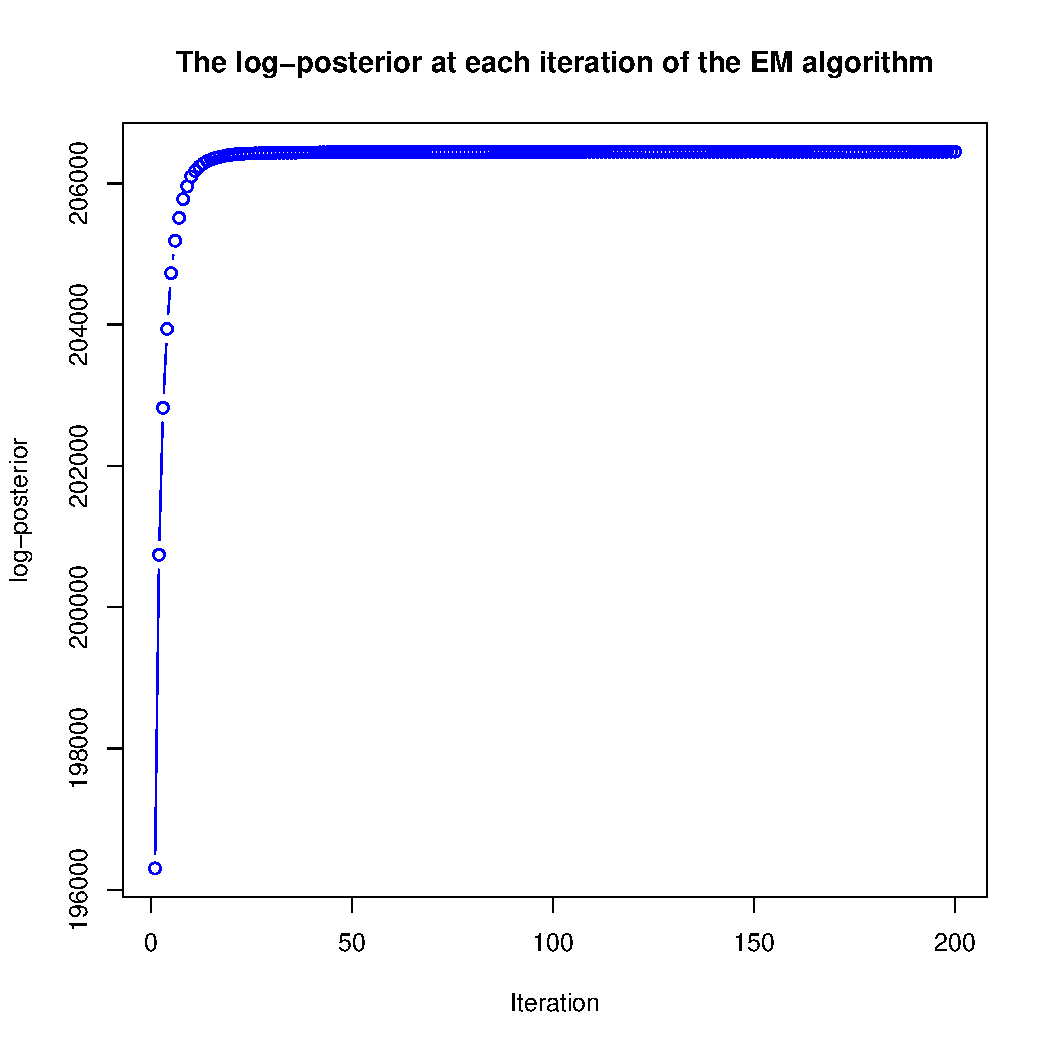
\includegraphics[width=0.6\textwidth]{figure/emconverge-1} 

\end{knitrout}

\caption{Plot of the log-posterior at each iteration of the EM
  algorithm to demonstrate monotonicity and convergence}
  \label{figure::emconvergence}
\end{figure}

\clearpage

\section{Trace plots for assessing MCMC convergence}\label{app:mcmc}



\begin{figure}[ht]
  \centering
\begin{knitrout}
\definecolor{shadecolor}{rgb}{0.969, 0.969, 0.969}\color{fgcolor}
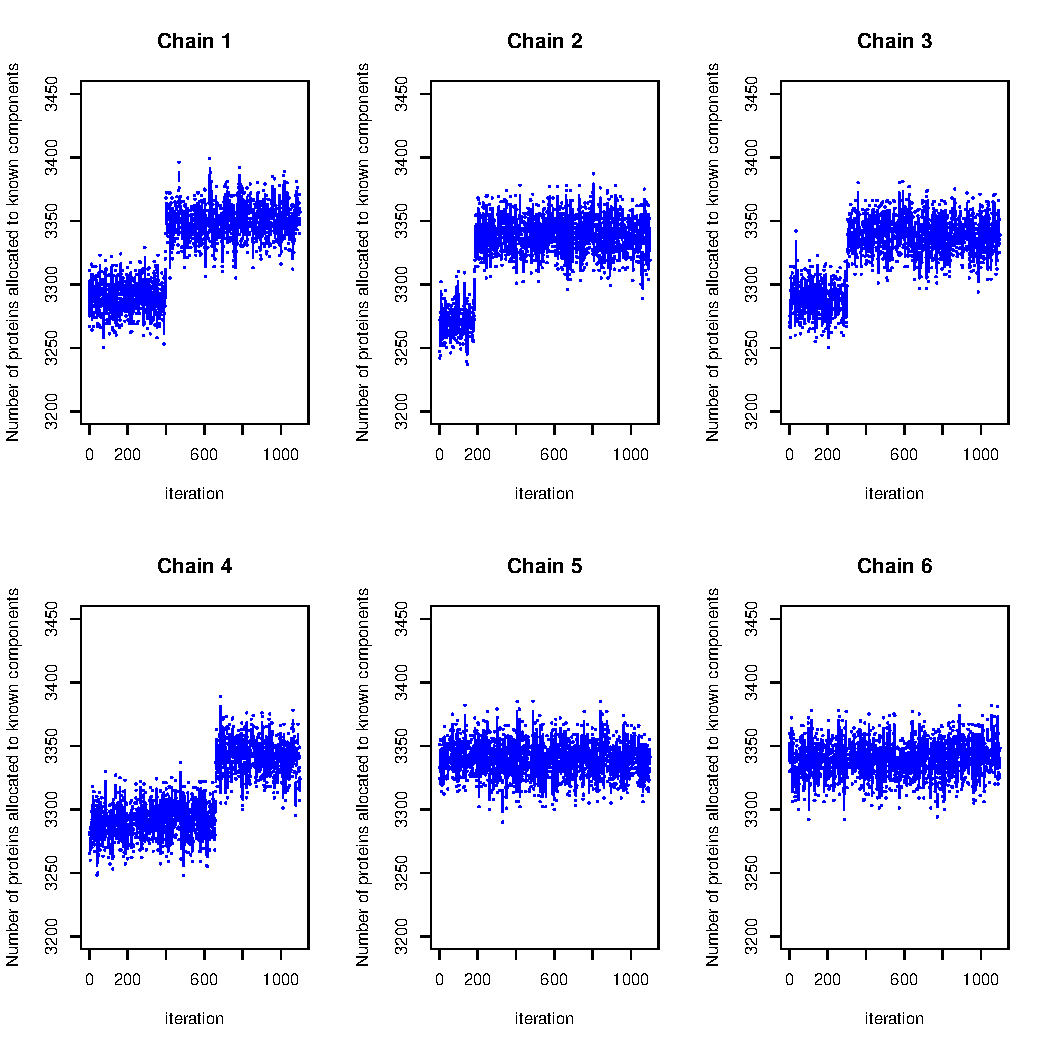
\includegraphics[width=0.75\textwidth]{figure/traceplots-1} 

\end{knitrout}
\caption{Trace plots of the number of proteins allocated to the known
  components in each of 6 parallel MCMC runs. Chain $4$ is discarded
  because of lack of convergence. $600$ samples are retained from
  remaining chains and pooled.}
  \label{figure::mcmcchains}
\end{figure}


\clearpage

\section{F1 t-tests}\label{app::ttestf1}




% latex table generated in R 3.5.1 by xtable 1.8-3 package
% Wed Oct 10 14:47:24 2018
\begin{table}[H]
\centering
\begin{tabular}{rrrr}
  \hline
 & SVM & KNN & MAP \\ 
  \hline
KNN & 2.7E-03 &  &  \\ 
  MAP & 3.3E-02 & 3.4E-01 &  \\ 
  MCMC & 3.4E-01 & 3.3E-02 & 2.3E-01 \\ 
   \hline
\end{tabular}
\caption{Adjusted P-values for pairwise T-tests for Macro F-1 score classifier evaluation on the Drosophila dataset} 
\end{table}
% latex table generated in R 3.5.1 by xtable 1.8-3 package
% Wed Oct 10 14:47:24 2018
\begin{table}[H]
\centering
\begin{tabular}{rrrr}
  \hline
 & SVM & KNN & MAP \\ 
  \hline
KNN & 1.2E-02 &  &  \\ 
  MAP & 2.7E-01 & 1.5E-01 &  \\ 
  MCMC & 4.9E-01 & 1.9E-03 & 1.1E-01 \\ 
   \hline
\end{tabular}
\caption{Adjusted P-values for pairwise T-tests for Macro F-1 score classifier evaluation on the Chicken DT40 dataset} 
\end{table}
% latex table generated in R 3.5.1 by xtable 1.8-3 package
% Wed Oct 10 14:47:24 2018
\begin{table}[H]
\centering
\begin{tabular}{rrrr}
  \hline
 & SVM & KNN & MAP \\ 
  \hline
KNN & 1.0E+00 &  &  \\ 
  MAP & 1.0E+00 & 1.0E+00 &  \\ 
  MCMC & 3.3E-01 & 6.0E-02 & 1.1E-05 \\ 
   \hline
\end{tabular}
\caption{Adjusted P-values for pairwise T-tests for Macro F-1 score classifier evaluation on the mouse dataset} 
\end{table}
% latex table generated in R 3.5.1 by xtable 1.8-3 package
% Wed Oct 10 14:47:24 2018
\begin{table}[H]
\centering
\begin{tabular}{rrrr}
  \hline
 & SVM & KNN & MAP \\ 
  \hline
KNN & 1.4E-35 &  &  \\ 
  MAP & 3.3E-06 & 6.7E-21 &  \\ 
  MCMC & 8.0E-59 & 3.2E-91 & 2.4E-70 \\ 
   \hline
\end{tabular}
\caption{Adjusted P-values for pairwise T-tests for Macro F-1 score classifier evaluation on the HeLa dataset} 
\end{table}
% latex table generated in R 3.5.1 by xtable 1.8-3 package
% Wed Oct 10 14:47:24 2018
\begin{table}[H]
\centering
\begin{tabular}{rrrr}
  \hline
 & SVM & KNN & MAP \\ 
  \hline
KNN & 1.3E-02 &  &  \\ 
  MAP & 4.3E-04 & 3.3E-09 &  \\ 
  MCMC & 5.8E-01 & 3.5E-03 & 3.1E-03 \\ 
   \hline
\end{tabular}
\caption{Adjusted P-values for pairwise T-tests for Macro F-1 score classifier evaluation on the U2-OS dataset} 
\end{table}
% latex table generated in R 3.5.1 by xtable 1.8-3 package
% Wed Oct 10 14:47:24 2018
\begin{table}[H]
\centering
\begin{tabular}{rrrr}
  \hline
 & SVM & KNN & MAP \\ 
  \hline
KNN & 2.2E-08 &  &  \\ 
  MAP & 1.0E-34 & 6.8E-14 &  \\ 
  MCMC & 7.4E-05 & 5.3E-02 & 1.0E-20 \\ 
   \hline
\end{tabular}
\caption{Adjusted P-values for pairwise T-tests for Macro F-1 score classifier evaluation on the HeLa wild (Hirst et al.) dataset} 
\end{table}
% latex table generated in R 3.5.1 by xtable 1.8-3 package
% Wed Oct 10 14:47:24 2018
\begin{table}[H]
\centering
\begin{tabular}{rrrr}
  \hline
 & SVM & KNN & MAP \\ 
  \hline
KNN & 5.3E-02 &  &  \\ 
  MAP & 1.7E-23 & 7.9E-27 &  \\ 
  MCMC & 9.1E-02 & 5.8E-04 & 1.8E-19 \\ 
   \hline
\end{tabular}
\caption{Adjusted P-values for pairwise T-tests for Macro F-1 score classifier evaluation on the HeLa KO1 (Hirst et al.) dataset} 
\end{table}
% latex table generated in R 3.5.1 by xtable 1.8-3 package
% Wed Oct 10 14:47:24 2018
\begin{table}[H]
\centering
\begin{tabular}{rrrr}
  \hline
 & SVM & KNN & MAP \\ 
  \hline
KNN & 1.3E-01 &  &  \\ 
  MAP & 1.1E-55 & 1.1E-55 &  \\ 
  MCMC & 1.0E-18 & 6.3E-22 & 2.0E-26 \\ 
   \hline
\end{tabular}
\caption{Adjusted P-values for pairwise T-tests for Macro F-1 score classifier evaluation on the HeLa KO2 (Hirst et al.) dataset} 
\end{table}
% latex table generated in R 3.5.1 by xtable 1.8-3 package
% Wed Oct 10 14:47:24 2018
\begin{table}[H]
\centering
\begin{tabular}{rrrr}
  \hline
 & SVM & KNN & MAP \\ 
  \hline
KNN & 9.6E-02 &  &  \\ 
  MAP & 4.1E-07 & 1.1E-09 &  \\ 
  MCMC & 2.8E-27 & 1.0E-28 & 6.3E-10 \\ 
   \hline
\end{tabular}
\caption{Adjusted P-values for pairwise T-tests for Macro F-1 score classifier evaluation on the Primary Fibroblasts Mock 24hpi dataset} 
\end{table}
% latex table generated in R 3.5.1 by xtable 1.8-3 package
% Wed Oct 10 14:47:24 2018
\begin{table}[H]
\centering
\begin{tabular}{rrrr}
  \hline
 & SVM & KNN & MAP \\ 
  \hline
KNN & 6.6E-07 &  &  \\ 
  MAP & 1.3E-10 & 2.0E-01 &  \\ 
  MCMC & 1.6E-05 & 2.0E-01 & 6.2E-03 \\ 
   \hline
\end{tabular}
\caption{Adjusted P-values for pairwise T-tests for Macro F-1 score classifier evaluation on the Primary Fibroblasts Mock 48hpi dataset} 
\end{table}
% latex table generated in R 3.5.1 by xtable 1.8-3 package
% Wed Oct 10 14:47:24 2018
\begin{table}[H]
\centering
\begin{tabular}{rrrr}
  \hline
 & SVM & KNN & MAP \\ 
  \hline
KNN & 3.9E-03 &  &  \\ 
  MAP & 9.5E-01 & 8.6E-03 &  \\ 
  MCMC & 6.4E-02 & 3.0E-01 & 8.6E-02 \\ 
   \hline
\end{tabular}
\caption{Adjusted P-values for pairwise T-tests for Macro F-1 score classifier evaluation on the Primary Fibroblasts Mock 72hpi dataset} 
\end{table}
% latex table generated in R 3.5.1 by xtable 1.8-3 package
% Wed Oct 10 14:47:24 2018
\begin{table}[H]
\centering
\begin{tabular}{rrrr}
  \hline
 & SVM & KNN & MAP \\ 
  \hline
KNN & 8.6E-03 &  &  \\ 
  MAP & 1.1E-02 & 8.6E-01 &  \\ 
  MCMC & 3.7E-06 & 1.6E-02 & 3.3E-02 \\ 
   \hline
\end{tabular}
\caption{Adjusted P-values for pairwise T-tests for Macro F-1 score classifier evaluation on the Primary Fibroblasts Mock 96hpi dataset} 
\end{table}
% latex table generated in R 3.5.1 by xtable 1.8-3 package
% Wed Oct 10 14:47:24 2018
\begin{table}[H]
\centering
\begin{tabular}{rrrr}
  \hline
 & SVM & KNN & MAP \\ 
  \hline
KNN & 1.9E-23 &  &  \\ 
  MAP & 1.4E-02 & 2.3E-34 &  \\ 
  MCMC & 3.8E-07 & 1.6E-81 & 2.0E-02 \\ 
   \hline
\end{tabular}
\caption{Adjusted P-values for pairwise T-tests for Macro F-1 score classifier evaluation on the Primary Fibroblasts Mock 120hpi dataset} 
\end{table}
% latex table generated in R 3.5.1 by xtable 1.8-3 package
% Wed Oct 10 14:47:24 2018
\begin{table}[H]
\centering
\begin{tabular}{rrrr}
  \hline
 & SVM & KNN & MAP \\ 
  \hline
KNN & 4.6E-01 &  &  \\ 
  MAP & 2.6E-05 & 1.7E-04 &  \\ 
  MCMC & 1.7E-04 & 1.3E-03 & 5.5E-01 \\ 
   \hline
\end{tabular}
\caption{Adjusted P-values for pairwise T-tests for Macro F-1 score classifier evaluation on the Primary Fibroblasts HCMV 24hpi dataset} 
\end{table}
% latex table generated in R 3.5.1 by xtable 1.8-3 package
% Wed Oct 10 14:47:24 2018
\begin{table}[H]
\centering
\begin{tabular}{rrrr}
  \hline
 & SVM & KNN & MAP \\ 
  \hline
KNN & 1.0E-02 &  &  \\ 
  MAP & 4.6E-01 & 1.5E-03 &  \\ 
  MCMC & 1.2E-02 & 7.3E-01 & 1.5E-03 \\ 
   \hline
\end{tabular}
\caption{Adjusted P-values for pairwise T-tests for Macro F-1 score classifier evaluation on the Primary Fibroblasts HCMV 48hpi dataset} 
\end{table}
% latex table generated in R 3.5.1 by xtable 1.8-3 package
% Wed Oct 10 14:47:24 2018
\begin{table}[H]
\centering
\begin{tabular}{rrrr}
  \hline
 & SVM & KNN & MAP \\ 
  \hline
KNN & 5.5E-02 &  &  \\ 
  MAP & 9.5E-06 & 3.4E-02 &  \\ 
  MCMC & 1.1E-01 & 6.2E-01 & 6.4E-03 \\ 
   \hline
\end{tabular}
\caption{Adjusted P-values for pairwise T-tests for Macro F-1 score classifier evaluation on the Primary Fibroblasts HCMV 72hpi dataset} 
\end{table}
% latex table generated in R 3.5.1 by xtable 1.8-3 package
% Wed Oct 10 14:47:24 2018
\begin{table}[H]
\centering
\begin{tabular}{rrrr}
  \hline
 & SVM & KNN & MAP \\ 
  \hline
KNN & 2.8E-01 &  &  \\ 
  MAP & 2.6E-09 & 7.2E-08 &  \\ 
  MCMC & 4.2E-10 & 5.6E-09 & 5.7E-01 \\ 
   \hline
\end{tabular}
\caption{Adjusted P-values for pairwise T-tests for Macro F-1 score classifier evaluation on the Primary Fibroblasts HCMV 96hpi dataset} 
\end{table}
% latex table generated in R 3.5.1 by xtable 1.8-3 package
% Wed Oct 10 14:47:24 2018
\begin{table}[H]
\centering
\begin{tabular}{rrrr}
  \hline
 & SVM & KNN & MAP \\ 
  \hline
KNN & 2.3E-04 &  &  \\ 
  MAP & 7.1E-04 & 3.8E-10 &  \\ 
  MCMC & 1.4E-01 & 5.7E-02 & 6.0E-05 \\ 
   \hline
\end{tabular}
\caption{Adjusted P-values for pairwise T-tests for Macro F-1 score classifier evaluation on the Primary Fibroblasts HCMV 120hpi dataset} 
\end{table}
% latex table generated in R 3.5.1 by xtable 1.8-3 package
% Wed Oct 10 14:47:24 2018
\begin{table}[H]
\centering
\begin{tabular}{rrrr}
  \hline
 & SVM & KNN & MAP \\ 
  \hline
KNN & 6.7E-06 &  &  \\ 
  MAP & 6.3E-05 & 4.4E-01 &  \\ 
  MCMC & 4.4E-01 & 6.7E-06 & 8.3E-05 \\ 
   \hline
\end{tabular}
\caption{Adjusted P-values for pairwise T-tests for Macro F-1 score classifier evaluation on the E14TG2a dataset} 
\end{table}


\clearpage

\section{Quadratic loss t-tests}




% latex table generated in R 3.5.1 by xtable 1.8-3 package
% Wed Oct 10 14:47:24 2018
\begin{table}[H]
\centering
\begin{tabular}{rrrr}
  \hline
 & SVM & KNN & MAP \\ 
  \hline
KNN & 5.9E-13 &  &  \\ 
  MAP & 1.1E-04 & 9.6E-124 &  \\ 
  MCMC & 2.2E-23 & 3.3E-58 & 5.9E-171 \\ 
   \hline
\end{tabular}
\caption{Adjusted P-values for pairwise T-tests for Quadratic Loss classifier evaluation on the Drosphila dataset} 
\end{table}
% latex table generated in R 3.5.1 by xtable 1.8-3 package
% Wed Oct 10 14:47:24 2018
\begin{table}[H]
\centering
\begin{tabular}{rrrr}
  \hline
 & SVM & KNN & MAP \\ 
  \hline
KNN & 3.2E-08 &  &  \\ 
  MAP & 1.7E-26 & 1.3E-128 &  \\ 
  MCMC & 4.2E-13 & 8.8E-37 & 7.0E-135 \\ 
   \hline
\end{tabular}
\caption{Adjusted P-values for pairwise T-tests for Quadratic Loss classifier evaluation on the Chicken DT40 dataset} 
\end{table}
% latex table generated in R 3.5.1 by xtable 1.8-3 package
% Wed Oct 10 14:47:24 2018
\begin{table}[H]
\centering
\begin{tabular}{rrrr}
  \hline
 & SVM & KNN & MAP \\ 
  \hline
KNN & 5.5E-14 &  &  \\ 
  MAP & 3.0E-25 & 6.3E-128 &  \\ 
  MCMC & 7.4E-26 & 1.7E-129 & 1.6E-14 \\ 
   \hline
\end{tabular}
\caption{Adjusted P-values for pairwise T-tests for Quadratic Loss classifier evaluation on the mouse dataset} 
\end{table}
% latex table generated in R 3.5.1 by xtable 1.8-3 package
% Wed Oct 10 14:47:24 2018
\begin{table}[H]
\centering
\begin{tabular}{rrrr}
  \hline
 & SVM & KNN & MAP \\ 
  \hline
KNN & 1.2E-02 &  &  \\ 
  MAP & 9.4E-07 & 7.4E-86 &  \\ 
  MCMC & 5.5E-08 & 2.7E-89 & 2.4E-12 \\ 
   \hline
\end{tabular}
\caption{Adjusted P-values for pairwise T-tests for Quadratic Loss classifier evaluation on the HeLa dataset} 
\end{table}
% latex table generated in R 3.5.1 by xtable 1.8-3 package
% Wed Oct 10 14:47:24 2018
\begin{table}[H]
\centering
\begin{tabular}{rrrr}
  \hline
 & SVM & KNN & MAP \\ 
  \hline
KNN & 6.8E-02 &  &  \\ 
  MAP & 7.4E-17 & 1.1E-73 &  \\ 
  MCMC & 1.4E-20 & 6.7E-81 & 8.3E-41 \\ 
   \hline
\end{tabular}
\caption{Adjusted P-values for pairwise T-tests for Quadratic Loss classifier evaluation on the U2-OS dataset} 
\end{table}
% latex table generated in R 3.5.1 by xtable 1.8-3 package
% Wed Oct 10 14:47:24 2018
\begin{table}[H]
\centering
\begin{tabular}{rrrr}
  \hline
 & SVM & KNN & MAP \\ 
  \hline
KNN & 2.3E-92 &  &  \\ 
  MAP & 9.0E-13 & 2.4E-83 &  \\ 
  MCMC & 6.6E-19 & 3.0E-81 & 1.1E-01 \\ 
   \hline
\end{tabular}
\caption{Adjusted P-values for pairwise T-tests for Quadratic Loss classifier evaluation on the HeLa wild (Hirst et al.) dataset} 
\end{table}
% latex table generated in R 3.5.1 by xtable 1.8-3 package
% Wed Oct 10 14:47:24 2018
\begin{table}[H]
\centering
\begin{tabular}{rrrr}
  \hline
 & SVM & KNN & MAP \\ 
  \hline
KNN & 5.2E-97 &  &  \\ 
  MAP & 1.4E-02 & 1.2E-90 &  \\ 
  MCMC & 2.3E-09 & 7.0E-95 & 2.2E-02 \\ 
   \hline
\end{tabular}
\caption{Adjusted P-values for pairwise T-tests for Quadratic Loss classifier evaluation on the HeLa KO1 (Hirst et al.) dataset} 
\end{table}
% latex table generated in R 3.5.1 by xtable 1.8-3 package
% Wed Oct 10 14:47:24 2018
\begin{table}[H]
\centering
\begin{tabular}{rrrr}
  \hline
 & SVM & KNN & MAP \\ 
  \hline
KNN & 8.9E-93 &  &  \\ 
  MAP & 3.1E-01 & 8.1E-91 &  \\ 
  MCMC & 9.0E-06 & 1.5E-83 & 8.9E-05 \\ 
   \hline
\end{tabular}
\caption{Adjusted P-values for pairwise T-tests for Quadratic Loss classifier evaluation on the HeLa KO2 (Hirst et al.) dataset} 
\end{table}
% latex table generated in R 3.5.1 by xtable 1.8-3 package
% Wed Oct 10 14:47:24 2018
\begin{table}[H]
\centering
\begin{tabular}{rrrr}
  \hline
 & SVM & KNN & MAP \\ 
  \hline
KNN & 6.1E-13 &  &  \\ 
  MAP & 1.4E-18 & 4.4E-81 &  \\ 
  MCMC & 3.2E-18 & 7.2E-77 & 5.9E-03 \\ 
   \hline
\end{tabular}
\caption{Adjusted P-values for pairwise T-tests for Quadratic Loss classifier evaluation on the Primary Fibroblasts Mock 24hpi dataset} 
\end{table}
% latex table generated in R 3.5.1 by xtable 1.8-3 package
% Wed Oct 10 14:47:24 2018
\begin{table}[H]
\centering
\begin{tabular}{rrrr}
  \hline
 & SVM & KNN & MAP \\ 
  \hline
KNN & 6.1E-18 &  &  \\ 
  MAP & 3.6E-24 & 2.2E-57 &  \\ 
  MCMC & 1.4E-24 & 3.6E-61 & 3.6E-04 \\ 
   \hline
\end{tabular}
\caption{Adjusted P-values for pairwise T-tests for Quadratic Loss classifier evaluation on the Primary Fibroblasts Mock 48hpi dataset} 
\end{table}
% latex table generated in R 3.5.1 by xtable 1.8-3 package
% Wed Oct 10 14:47:24 2018
\begin{table}[H]
\centering
\begin{tabular}{rrrr}
  \hline
 & SVM & KNN & MAP \\ 
  \hline
KNN & 1.2E-15 &  &  \\ 
  MAP & 4.5E-23 & 2.5E-89 &  \\ 
  MCMC & 4.2E-23 & 5.1E-91 & 4.4E-01 \\ 
   \hline
\end{tabular}
\caption{Adjusted P-values for pairwise T-tests for Quadratic Loss classifier evaluation on the Primary Fibroblasts Mock 72hpi dataset} 
\end{table}
% latex table generated in R 3.5.1 by xtable 1.8-3 package
% Wed Oct 10 14:47:24 2018
\begin{table}[H]
\centering
\begin{tabular}{rrrr}
  \hline
 & SVM & KNN & MAP \\ 
  \hline
KNN & 1.8E-13 &  &  \\ 
  MAP & 1.4E-20 & 3.6E-126 &  \\ 
  MCMC & 5.0E-20 & 1.5E-109 & 5.3E-07 \\ 
   \hline
\end{tabular}
\caption{Adjusted P-values for pairwise T-tests for Quadratic Loss classifier evaluation on the Primary Fibroblasts Mock 96hpi dataset} 
\end{table}
% latex table generated in R 3.5.1 by xtable 1.8-3 package
% Wed Oct 10 14:47:24 2018
\begin{table}[H]
\centering
\begin{tabular}{rrrr}
  \hline
 & SVM & KNN & MAP \\ 
  \hline
KNN & 6.7E-14 &  &  \\ 
  MAP & 1.0E-19 & 2.6E-45 &  \\ 
  MCMC & 8.0E-20 & 2.4E-45 & 2.5E-02 \\ 
   \hline
\end{tabular}
\caption{Adjusted P-values for pairwise T-tests for Quadratic Loss classifier evaluation on the Primary Fibroblasts Mock 120hpi dataset} 
\end{table}
% latex table generated in R 3.5.1 by xtable 1.8-3 package
% Wed Oct 10 14:47:24 2018
\begin{table}[H]
\centering
\begin{tabular}{rrrr}
  \hline
 & SVM & KNN & MAP \\ 
  \hline
KNN & 6.0E-22 &  &  \\ 
  MAP & 2.8E-27 & 6.4E-53 &  \\ 
  MCMC & 1.4E-27 & 1.5E-56 & 3.0E-03 \\ 
   \hline
\end{tabular}
\caption{Adjusted P-values for pairwise T-tests for Quadratic Loss classifier evaluation on the Primary Fibroblasts HCMV 24hpi dataset} 
\end{table}
% latex table generated in R 3.5.1 by xtable 1.8-3 package
% Wed Oct 10 14:47:24 2018
\begin{table}[H]
\centering
\begin{tabular}{rrrr}
  \hline
 & SVM & KNN & MAP \\ 
  \hline
KNN & 1.9E-26 &  &  \\ 
  MAP & 1.3E-33 & 2.7E-84 &  \\ 
  MCMC & 1.3E-33 & 2.7E-84 & 6.0E-01 \\ 
   \hline
\end{tabular}
\caption{Adjusted P-values for pairwise T-tests for Quadratic Loss classifier evaluation on the Primary Fibroblasts HCMV 48hpi dataset} 
\end{table}
% latex table generated in R 3.5.1 by xtable 1.8-3 package
% Wed Oct 10 14:47:24 2018
\begin{table}[H]
\centering
\begin{tabular}{rrrr}
  \hline
 & SVM & KNN & MAP \\ 
  \hline
KNN & 6.3E-20 &  &  \\ 
  MAP & 1.9E-25 & 2.7E-57 &  \\ 
  MCMC & 1.2E-25 & 3.4E-58 & 1.5E-02 \\ 
   \hline
\end{tabular}
\caption{Adjusted P-values for pairwise T-tests for Quadratic Loss classifier evaluation on the Primary Fibroblasts HCMV 72hpi dataset} 
\end{table}
% latex table generated in R 3.5.1 by xtable 1.8-3 package
% Wed Oct 10 14:47:24 2018
\begin{table}[H]
\centering
\begin{tabular}{rrrr}
  \hline
 & SVM & KNN & MAP \\ 
  \hline
KNN & 1.7E-25 &  &  \\ 
  MAP & 9.3E-32 & 1.9E-56 &  \\ 
  MCMC & 9.3E-32 & 1.2E-54 & 7.1E-01 \\ 
   \hline
\end{tabular}
\caption{Adjusted P-values for pairwise T-tests for Quadratic Loss classifier evaluation on the Primary Fibroblasts HCMV 96hpi dataset} 
\end{table}
% latex table generated in R 3.5.1 by xtable 1.8-3 package
% Wed Oct 10 14:47:24 2018
\begin{table}[H]
\centering
\begin{tabular}{rrrr}
  \hline
 & SVM & KNN & MAP \\ 
  \hline
KNN & 6.5E-25 &  &  \\ 
  MAP & 5.3E-32 & 1.1E-71 &  \\ 
  MCMC & 7.1E-32 & 8.4E-71 & 5.7E-02 \\ 
   \hline
\end{tabular}
\caption{Adjusted P-values for pairwise T-tests for Quadratic Loss classifier evaluation on the Primary Fibroblasts HCMV 120hpi dataset} 
\end{table}
% latex table generated in R 3.5.1 by xtable 1.8-3 package
% Wed Oct 10 14:47:24 2018
\begin{table}[H]
\centering
\begin{tabular}{rrrr}
  \hline
 & SVM & KNN & MAP \\ 
  \hline
KNN & 4.7E-04 &  &  \\ 
  MAP & 4.7E-21 & 1.5E-103 &  \\ 
  MCMC & 3.3E-12 & 1.8E-57 & 1.3E-137 \\ 
   \hline
\end{tabular}
\caption{Adjusted P-values for pairwise T-tests for Quadratic Loss classifier evaluation on the E14TG2a dataset} 
\end{table}


\clearpage

\section{GO enrichment analysis figures}



\begin{figure}[h]
  \centering
  \begin{subfigure}[t]{0.5\textwidth}
    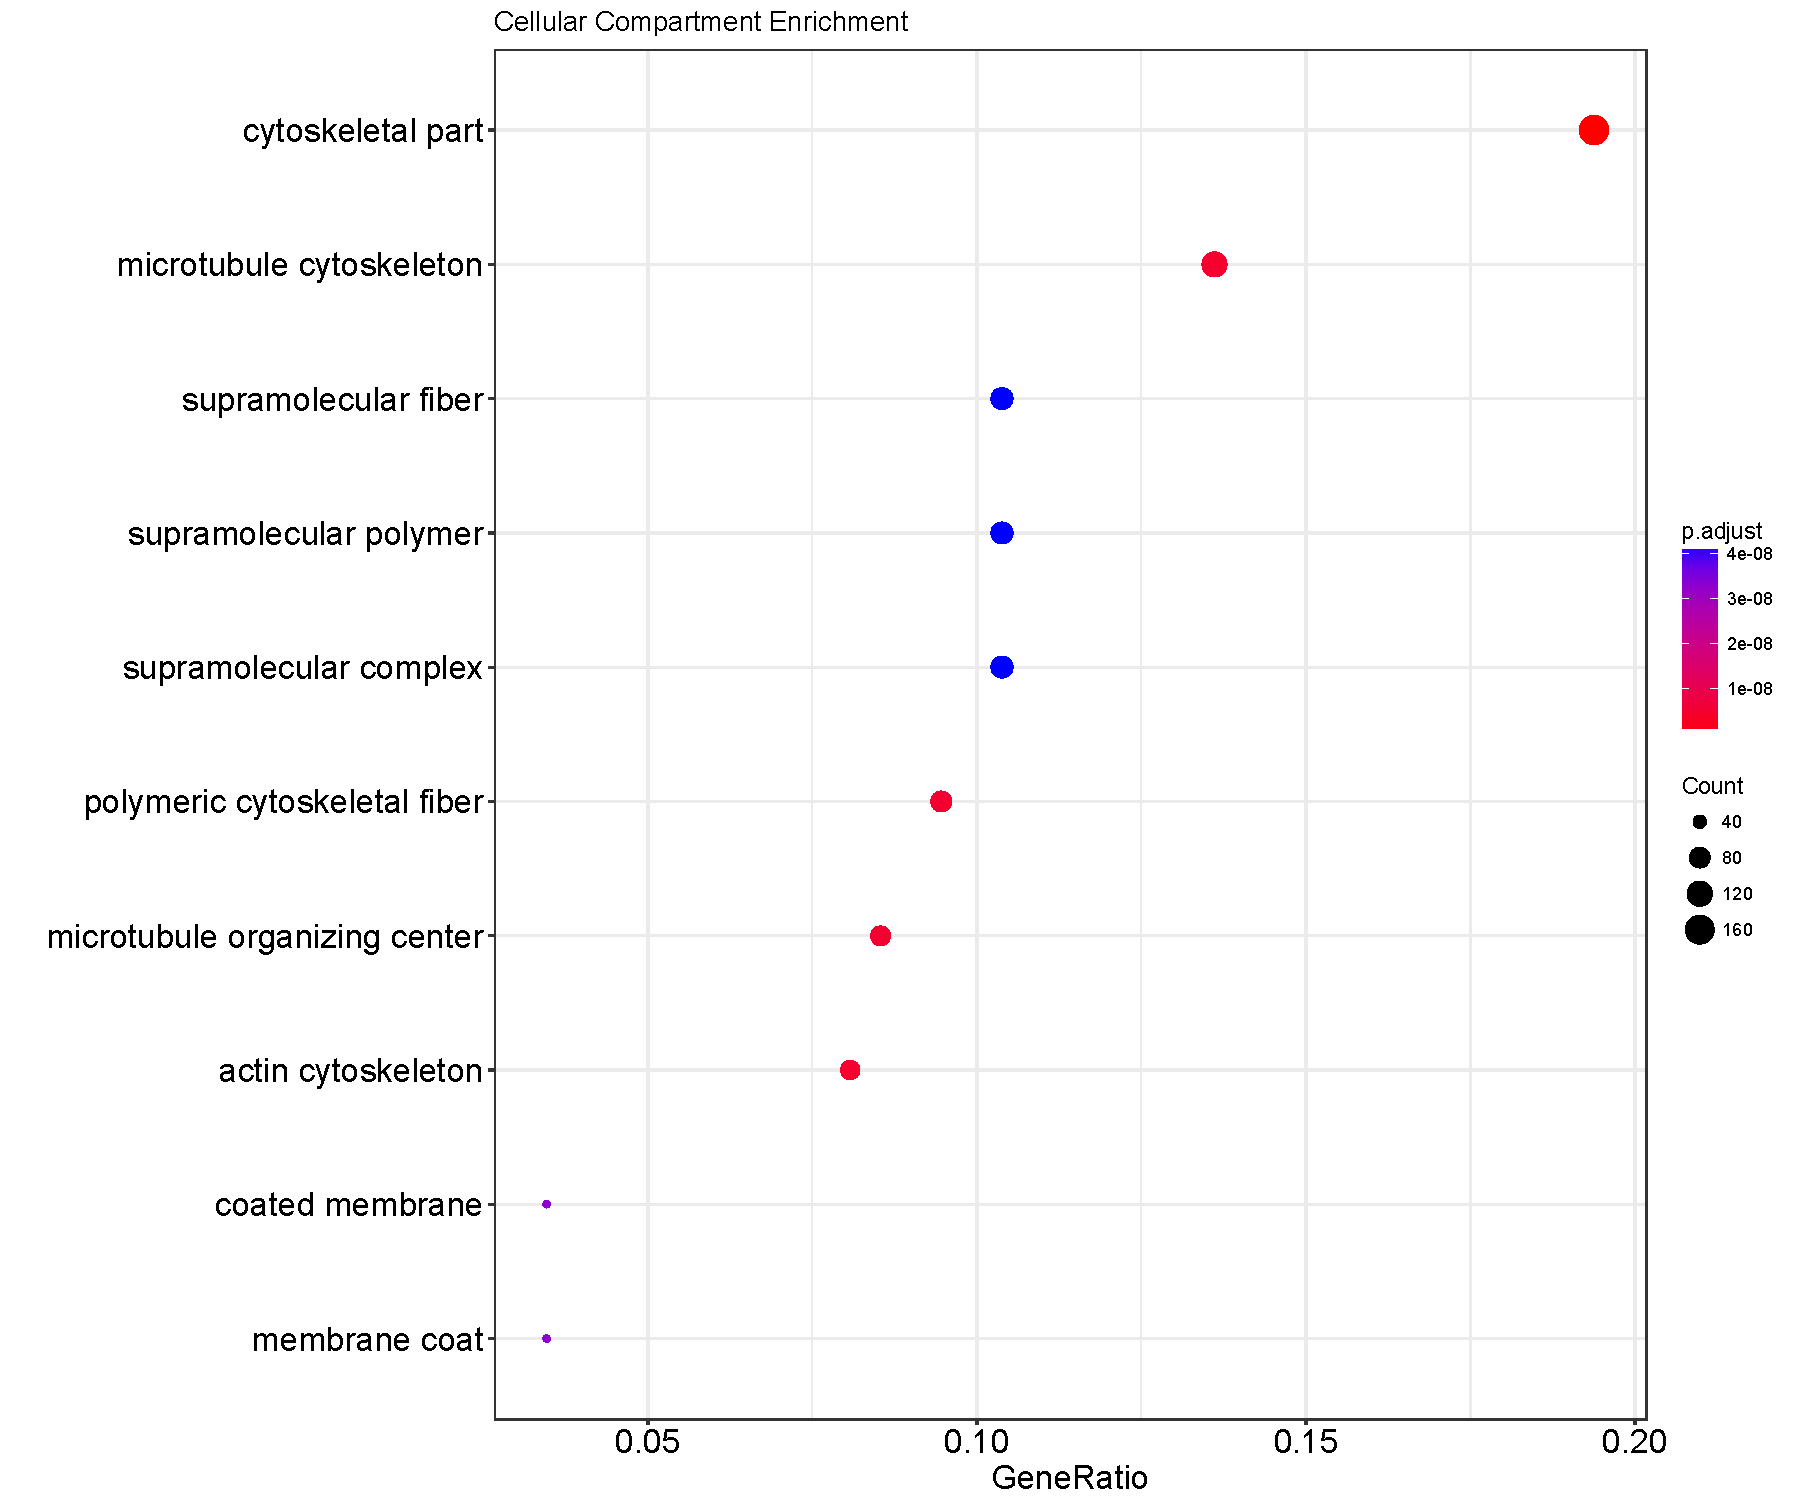
\includegraphics[width=\textwidth]{CCenrich.pdf}
  \end{subfigure}%
  \begin{subfigure}[t]{0.5\textwidth}
    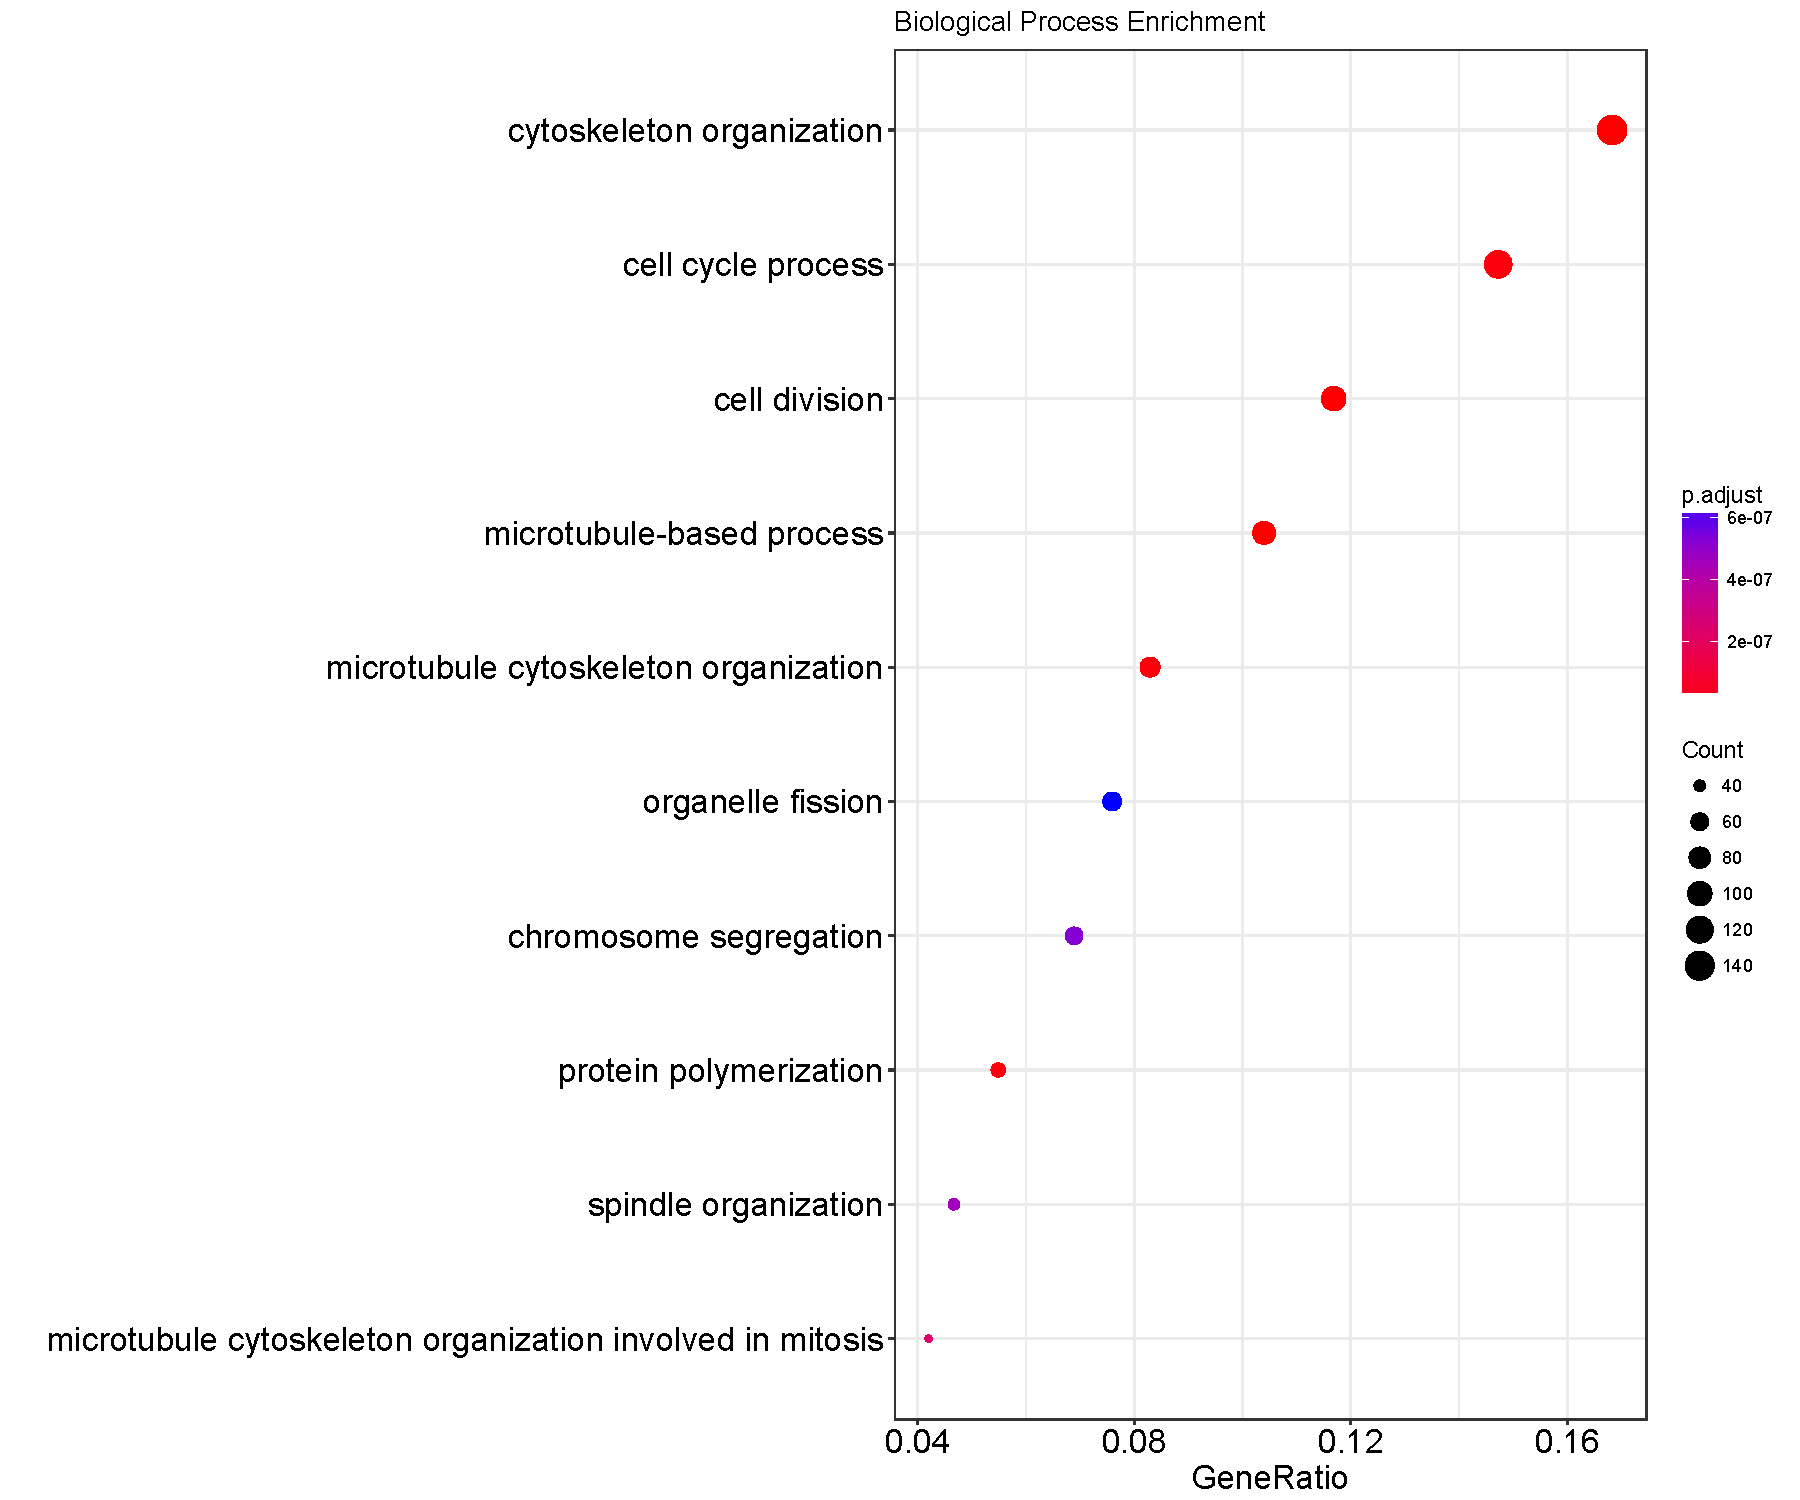
\includegraphics[width=\textwidth]{BPenrich.pdf}
  \end{subfigure}%
~

  \begin{subfigure}[t]{0.5\textwidth}
    \centering
    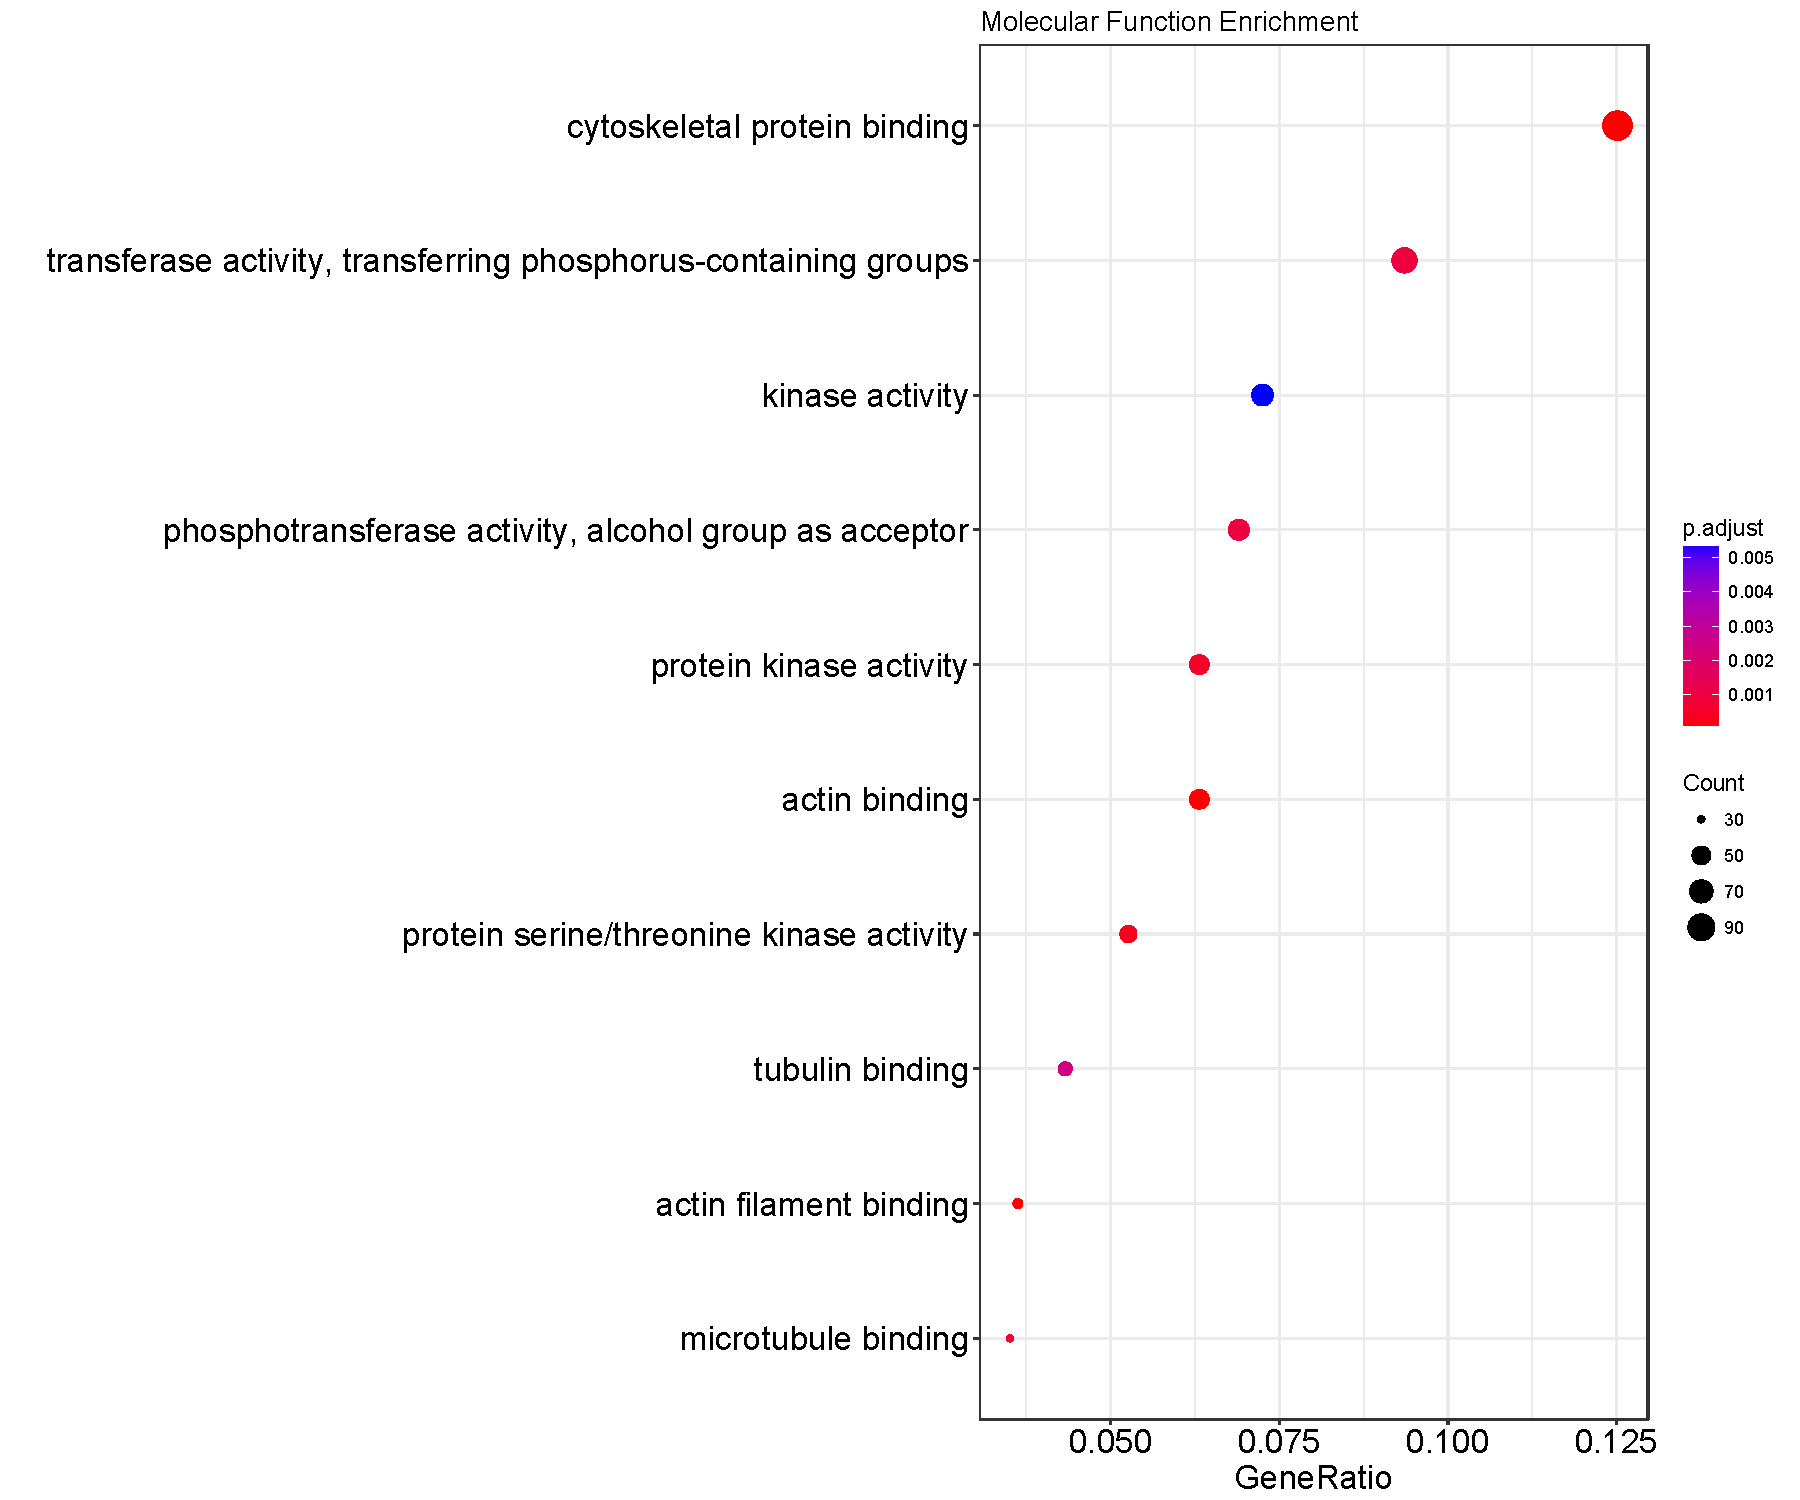
\includegraphics[width=\textwidth]{MFenrich.pdf}
  \end{subfigure}
  \caption{Gene Ontology over representation analysis on outlier
    proteins - that is proteins allocated with less than probability
    $0.95$. We analyse the enrichment of terms in the cellular
    compartment, biological process, and molecular function
    ontologies. We display the top 10 significant results in the
    dotplots.}
  \label{fig:GOenrich}
\end{figure}

\clearpage

\section{Comparison of MCMC and MAP allocations}

\begin{figure}[ht]
\centering
\begin{knitrout}
\definecolor{shadecolor}{rgb}{0.969, 0.969, 0.969}\color{fgcolor}
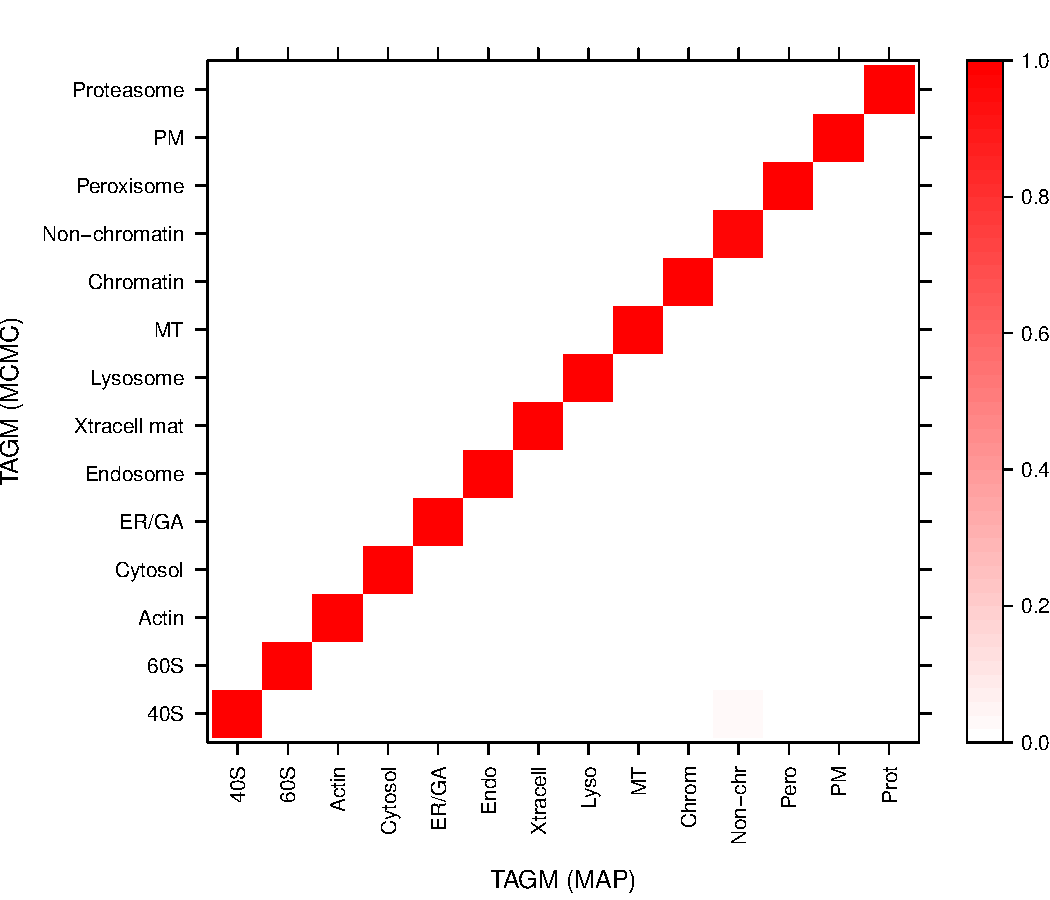
\includegraphics[width=\maxwidth]{figure/app8-heatmap-1} 

\end{knitrout}
\caption{A heatmap representation of a contingency table comparing allocation produced by
MCMC and MAP methods with posterior probability threshold set at $0.99$ for both methods.
The scale ranges from 0 to 1 with values indicating the proportion of assigned proteins to
that sub-cellular location. Values along the diagonal represent agreement between classifiers
whilst other values represent disagreement.
The allocations of proteins by both methods are in strong agreement.}
\end{figure}



\clearpage

\bibliographystyle{natbib}
\bibliography{BayesProt}


\end{document}
